\documentclass[twoside]{article}
\usepackage{graphicx}

%\usepackage[latin1]{inputenc}
\usepackage[utf8]{inputenc}
\usepackage[spanish]{babel}
\usepackage{amsmath, amsthm, amsfonts}
\usepackage{textcomp}
\usepackage[T1]{fontenc}
\usepackage{hyperref}
\usepackage{array}
\usepackage{MnSymbol}   % Para poder escribir el cuadrado negro

\usepackage{geometry}
    \geometry{a4paper,total={210mm,297mm},left=35mm,right=30mm,top=30mm,bottom=30mm,}

\usepackage{listings}

\usepackage{pgfplots}

\usepackage{tikz}
\usetikzlibrary{arrows,shapes,trees}

\title{\begin{center} 

\includegraphics[scale=0.3]{images/upc.jpg} 
\end{center} 
\vspace{1cm} 
Proyecto Final de Carrera\\
INGENIERÍA INDUSTRIAL \\
\vspace{1.5cm} 
\Huge{Control de un Quadcopter} 
\vspace{2cm} \\ 
Memoria}
%\author{Gabriel de la Cal Mendoza}
\date{}

\usepackage{fancyhdr}		%% Para cabezera de página

\pagestyle{fancy}

% \lhead[x1]{x2}
% \chead[y1]{y2}
% \rhead[LE,RO]{z2}
% \renewcommand{\headrulewidth}{0.5pt}

% \lfoot[a1]{b2}
% \cfoot[c1]{d2}
% \rfoot[LE,RO]{
\includegraphics[scale=0.1]{etseib.jpg}}
% \renewcommand{\footrulewidth}{0.5pt}

\fancyhead[LO,RE]{Quadcopter Control}
\fancyhead[LE,RO]{\thepage}
\fancyfoot[LE,RO]{
\includegraphics[scale=0.2]{images/etseib.jpg}}
\fancyfoot[C]{}

\begin{document}
\maketitle
\begin{center}
\large{
$\begin{array}{ll}
\mbox{Autor:} & \mbox{Gabriel de la Cal Mendoza} \\
\mbox{Director:} & \mbox{Manel Velasco Garcia} \\
\mbox{Convocatoria:} & \mbox{Fecha a presentar}
\end{array}$}
\\ \vspace{2cm} \Large{Escola Tècnica Superior d'Enginyeria Industrial de Barcelona}\\ \vspace{1cm}

\includegraphics[scale=0.4]{images/etseib.jpg}
\end{center}

\thispagestyle{empty}
\newpage
\begin{center}

\end{center}
\thispagestyle{empty}
\newpage
\setcounter{page}{1}

\section*{Resumen}

En el presente proyecto se ha tenido como meta el control de un Quadcopter cuyas piezas se han adquirido por partes. Para tal propósito se ha linealizado  el modelo no lineal calculado y controlado mediante un Regulador Lineal Cuadrático (LQR). El contenido de este trabajo esta organizado en 8 secciones y 4 secciones.\\

En la sección \ref{prefacio} se presentan los motivos por el que la elección del tema de este PFC queda justificado. También se mencionan requerimientos previos que se han requerido para no tener insalvables dificultades. \\
En la sección \ref{}



\newpage
\begin{center}

\end{center}
\thispagestyle{empty}
\newpage

\setcounter{page}{1}
\tableofcontents
\addcontentsline{toc}{section}{Resum}
\fancyhead[LE,RO]{3}
\fancyfoot[C]{}
\newpage
\fancyhead[LE,RO]{\thepage}
\setcounter{page}{4}
\listoffigures
\newpage

\section{Prefacio} \label{prefacio}
\subsection{Motivación}

La principal motivación de este proyecto es la de aplicar por uno mismo los conocimientos básicos adquiridos en la carrera, y más en particular en el área del control en haber cursado la intensificación de automática.\\

En plantear un tema para el proyecto rápidamente surgió la idea de realizarlo sobre el control de un sistema mecánico, y más en particular sobre uno que estuviera actualmente emergiendo tanto en mercados como en el campo de la investigación.\\ 

De entre las diferentes alternativas, un quadcopter es la más atractiva para el proyecto tanto por su simplicidad constructiva como por su no excesivo coste. Existen actualmente en el mercado infinidad de proveedores para los componentes necesarios para construir un quadcopter, con un gran abanico de opciones de entre las que escoger cada elemento como motores, baterías, electrónica, etc.\\

Las posibles aplicaciones son numerosas, tanto que aún no se han ni tan solo explotado todas las posibles. Como ejemplo: vigilancia de superficies abiertas, transporte de pequeños paquetes, herramienta de ocio, entre otras.\\

Entender el funcionamiento y familiarizarse con el mecanismo es una inquietud que se ha mantenido insatisfecha durante largo tiempo. Con este pretexto se pretende acabar de justificar la elección del tema de ésta pequeña gran empresa.

\subsection{Requerimientos previos}

Es necesario tener ciertos conocimientos mínimos en automática para poder controlar el quadcopter, así como la inquietud de aprender lo que sea necesario para cumplir, en la medida de lo posible, los objetivos iniciales del presente proyecto. \\

Nociones de mecánica son necesarias para elaborar e interpretar el sistema sobre el que se trabaje, así como sus resultados. Conocimientos del lenguaje $C$ son imprescindibles ya que el código del programa que realiza los cálculos está escrito en este mismo lenguaje. 

Para adaptar los elementos que componen el aparato y afianzarlos a la estructura (Frame)  del Quadcopter ha sido de gran ayuda contar con el servicio de una impresora 3D, creada por uno mismo. Finalmente, estar familiarizado con el argot y elementos de un Quadcopter, así como motores, emisoras de radio, entre otros es de ayuda. \\

Superar las dificultades que han surgido, teniendo en cuenta que el fin no justifica los medios, es la praxis que se ha aplicado a la hora de realizar éste trabajo. Finalmente, recordar reminiscencias de la carrera es siempre útil e interesante, así que conceptos adquiridos pero no utilizados se esperan aplicar.
 
\newpage
\section{Introducción} \label{intro}

Un Quadcopter es un vehículo volador no tripulado ($Unmanned \>Aerial\>Vehicle$ o $UAV$) que se caracteriza por tener quatro rotores a modo de actuadores en vez de dos como en el caso de los helicópteros. Este tipo de autogiro intenta obtener una flotabilidad estable y vuelo preciso balanceando las fuerzas producidas por los cuatro motores y surge de la necesidad de un aparato de vuelo de dimensiones reducidas y gran estabilidad, con prestaciones superiores a las de un helicóptero convencional. \\

\begin{figure}[h!]
\begin{center}
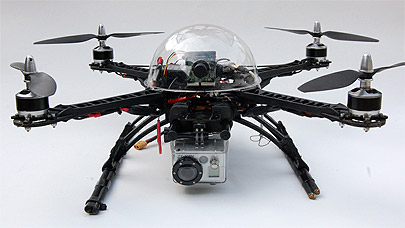
\includegraphics[scale=0.4]{images/quadcopter_example.jpg}
\caption{Quadcopter de ejemplo con cámara}
\end{center}
\end{figure}


Una de las ventajas que se obtiene con este cambio es la mayor capacidad de carga ya que es tienen 4 motores  para soportar el peso. La estabilidad del vehículo mejora en permitir aterrizajes y despegues verticales con una mayor maniobrabilidad. También puede trabajar en áreas de difícil acceso o más agresivas, como con lluvia y viento. \\

Esquemáticamente se puede representar como una estructura en $X$ con su centroide coincidiendo con el centro de masas i cuatro actuadores a las puntas de cada brazo, todos ellos apuntando en la misma dirección y sentido, pero con giros de aspa en sentido contrario, pero igual en lados opuestos.


\subsection{Estudio del arte}

En la actualidad el campo referente a estos aparatos se ha diversificado tanto que se pueden encontrar muchas variedades y tipos de Quadcopters. Se ha hecho mención del modelo de cuatro motores, pero bien pueden encontrarse de tres hasta 8 motores, sino más en casos más concretos. \\

\begin{figure}[h!]
\begin{center}
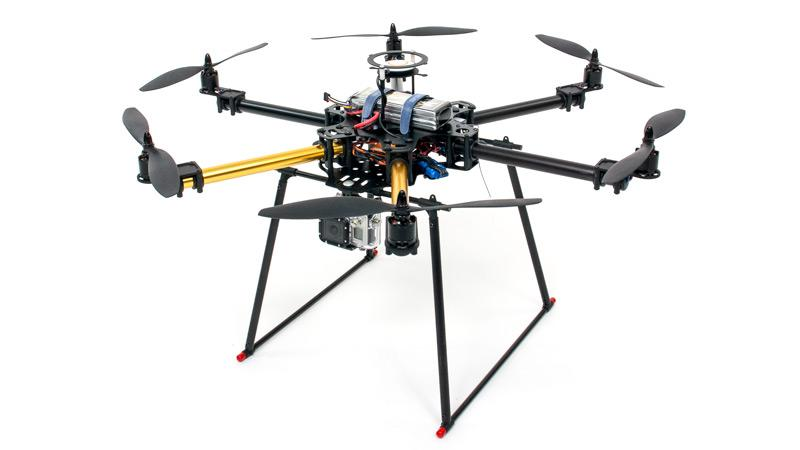
\includegraphics[scale=0.3]{images/6_armed_quadcopter.jpg}
\caption{Ejemplo de Quadcopter con 6 motores}
\end{center}
\end{figure}

Con el objetivo de desarrollar un $UAV$ que realice tareas de forma totalmente autónoma, se han diseñado sensores para estimar los estados del vehículo de manera más rápida y eficiente, así como diferentes estrategias para controlar la estabilidad y orientación del mismo. Se ha utilizado visión  por computador para realizar aterrizajes, detección de objetivos y navegación autónoma. También pueden combinarse diferentes técnicas con el uso del GPS para asegurar una buena odometría del aparato. \\

\subsection{Objetivos del proyecto}

La meta que se persigue es la de hacer planear un Quadcopter en direcciones horizontales. A la vez, éste es un excelente subterfugio para cumplir con otros objetivos relacionados con este fin como el control de motores, el inteligente uso de la electrónica y correcto diseño mecánico del aparato. Además, se espera haber ampliado la visión que uno tiene en cada campo. \\

De entre todas las disciplinas involucradas, se espera acabar familiarizado con las facetas relacionadas con la presente empresa para clarificar la relación entre los elementos que componen un Quadcopter.  A saber, se espera poder acabar entendiendo la electrónica, mecánica y conocimientos de control que reinan en el sistema. \\

En el caso de la electrónica se espera entender y poder implementar sencillos protocolos de comunicación, en este caso $I2C$ entre los sensores y la Raspberry Pi. Ésta misma es el centro neurálgico del Quadcopter, así que es esencial saber utilizarla como se requiere para que pueda recibir consignas, estados y enviar la correspondiente acción de control a los motores para que se llegue al estado final deseado. \\

Por parte de la mecánica, es primordial tener conocimientos sólidos de conceptos como el Teorema de la Cantidad de Movimiento y el de la conservación del Momento de Inercia, así como poder calcular el Lagrangiano ($\mathcal{L}$) para generar un modelo verosímil y que represente fidedignamente la realidad para que se desarrolle de manera efectiva el control. \\

Finalmente, y como más serio objetivo de toda esta aventura, es el de haber afianzado lo que se creía entendido en relación al control. Asimilar otros métodos de control aplicables a sistemas multilineales no contemplados en la carrera es un excitante reto que se espera haber superado con éxito. \\

Entonces, se entiende este trabajo como la causa de la motivación a cumplir con un objetivo multidisciplinar como puede serlo cualquiera en el campo de la robótica, en el que se debe tener constancia de muchos aspectos relevantes, como el de la economía. Poder tener idea de lo que cuesta un robot es de gran importancia si uno se embarca en un proyecto de envergadura, ya que se quiere que los pronósticos sobre el presupuesto cuadren con la futura realidad. 

\newpage
\section{Definición del modelo} \label{model}
\subsection{Definición de les variables}
Para caracterizar la planta con la que es trabajará, es necesario obtener un modelo del Quadcopter. Las constantes propias del modelo se dejaran en forma de parámetros a calibrar una vez se tenga el objeto físico. De esta manera el modelo será general para todo quadcopter que comparta la misma familia de parámetros.
Es necesario considerar dos marcos de referencia: el inercial formado por los ejes $x,y,z$ y el del cuerpo (Body) formado por los ejes $x_B,y_B,z_B$. El primero tiene la perspectiva de el observador en tierra, estático, mientras que el segundo es solidario a la estructura. Según la orientación de los ejes del cos con esta referencia se pueden dar los siguientes dos casos:
\begin{itemize}
\item \textbf{Cross type}: Los ejes de coordenadas coinciden con los brazos de la estructura ya que se tienen los actuadores a las puntas de cada brazo.
\item \textbf{X-type}: Los ejes y la estructura forman $45º$. Se tienen entonces dos motores en la parte delantera y dos en la trasera.
\end{itemize} 
Por ser más usual la primera opción, se decide utilizar la configuración $Cross type$ tal y como se tiene en la figura \ref{RefQuad}.
\begin{figure}[h!]
\centering
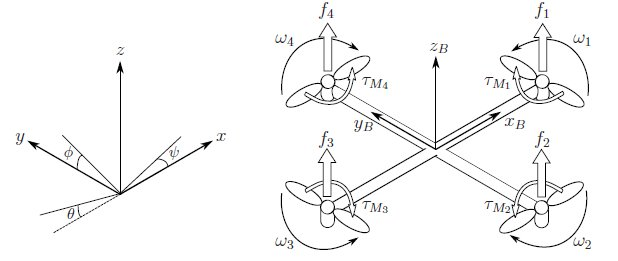
\includegraphics[scale=0.5]{images/quad.jpg}
\caption{Marcs de referència en el quadcopter}
\label{RefQuad}
\end{figure}\\
Se supone que el objeto es un rotor esférico, y por tanto su tensor de inercia es diagonal:
\begin{equation}\textbf{I}=\left[ \begin{array}{ccc}
I_{xx} & 0 & 0 \\
0 & I_{yy} & 0 \\
0 & 0 & I_{zz} 
\end{array} \right] \end{equation}
Se define la posición lineal absoluta con las coordenadas $x,y,z$ con vector $\pmb{\xi}$ e igualmente para la posición angular a partir de $\pmb{\eta}$ según:
\begin{equation} 
\pmb{\xi}=\left[ \begin{array}{ccc}
x\\
y\\
z \end{array} \right] ,\quad \pmb{\eta}=\left[ \begin{array}{ccc}
\phi\\
\theta\\
\psi \end{array} \right] , \quad \pmb{q}=\left[\begin{array}{c}
\pmb{\xi}\\
\pmb{\eta} \end{array} \right] 
\end{equation}

donde $\phi$ es el ángulo de cabeceo (Pitch), $\theta$ és el de balanceo (Roll) y $\psi$ el de guiñada (Yaw).\\
Para la orientación angular entre los dos marcos se tiene un sistema de referencia con ángulos Tait-Bryan, donde la matriz de transformación es:
\begin{equation}
\pmb{R}=\left[\begin{array}{ccc}
C_\psi C_\theta & C_\psi S_\theta S_\phi - S_\psi C_\phi & C_\psi S_\theta C_\phi + S_\psi S_\phi \\
S_\psi C_\theta & S_\psi S_\theta S_\phi + C_\psi C_\phi & S_\psi S_\theta C_\phi - C_\psi C_\phi \\
-S_\theta & C_\theta C_\phi & C_\theta C_\phi 
\end{array}\right]
\end{equation}
con $C_\phi=cos(\phi)$ i $S_\phi=sin(\phi)$.\newpage
Las velocidades lineales en el marco de referencia del cuerpo (Body Frame) se representen con el vector $v_B$ y las velocidades angulares con $\gamma$ según:
\begin{equation}
\pmb{v_B}=\left[\begin{array}{c}
v_{x,b}\\
v_{y,b}\\
v_{z,b}\\
\end{array}\right] \hspace{1cm} \pmb{\gamma}=\left[\begin{array}{c}
p\\
n\\
r
\end{array} \right]
\end{equation}
En cambio, las velocidades en el marco de referencia inercial (Inertial Frame)  se representan por $\dot{\eta}$ para las velocidades lineales y con $\dot{\xi}$ para las angulares: 
\begin{equation}
\pmb{\dot{\xi}}=\left[\begin{array}{c}
\dot{x} \\
\dot{y} \\
\dot{z}
\end{array} \right] \hspace{1cm} \pmb{\dot{\eta}}=\left[\begin{array}{c}
\dot{\psi} \\
\dot{\theta} \\
\dot{\psi}
\end{array} \right] 
\end{equation}
Ya que la derivada de los ángulos $\phi$, $\theta$ y $\psi$ no es el vector de velocidades angulares es necesario tener un cambio de base para relacionar el marco de referencia inercial con el del cuerpo con la matriz $W_\eta$:
\begin{equation}
\pmb{W_\eta}=\left[\begin{array}{ccc}
1 & 0 & -S_\theta \\
0 & C_\phi & C_\theta S_\phi \\
0 & -S_\phi & C_\theta C_\phi 
\end{array} \right] \hspace{0.5cm} amb \hspace{0.5cm} 
\pmb{\gamma}=\left[ \pmb{W_\eta} \right] \pmb{\dot{\eta}} 
\end{equation}
Las fuerzas de sustentación y velocidades angulares de los cuatro actuadores son $f_1,f_2,f_3,f_4$ i $w_1,w_2,w_3,w_4$ respectivamente. Siguiendo la orientación de la figura \ref{RefQuad}, con el objetivo de poder anular los momentos producidos en el eje $z_B$ (en el marco del cuerpo $B$) el sentido de giro de los actuadores  $4$ y $2$ son en el de las agujas del reloj (clockwise) y el de los $1$ y $3$ en sentido contrario (counterclockwise). \\

Interesa conocer qué fuerza y momento aportará cada motor dada una velocidad angular conocida. Se supone poder controlar la fuerza y momento ejercida por cada motor y cómo aproximación inicial se considera que están relacionados con la velocidad angular de la forma:
\begin{equation}
\begin{array}{l}
f_i=kw^2_i \\ 
\tau_{M_i}=bw^2_i
\end{array}
\end{equation}
Por tanto el empuje total $\pmb{T_B}$ proporcionado en la dirección $z_B$ y los momentos generados $\pmb{\tau_B}$ por los motores son:
\begin{equation}
\pmb{T_B}=k\left(\sum_{i=1}^{4}w^2_i \right)e_{z_B}=\left[ \begin{array}{c}
0 \\
0 \\
\displaystyle\sum_{i=1}^{4}f_i
\end{array} \right] 
\hspace{1cm} \pmb{\tau_B}=\left[ \begin{array}{c}
\tau_\phi \\
\tau_\theta \\
\tau_\psi
\end{array} \right] = \left[ \begin{array}{c}
l(f_4 - f_2) \\
l(f_3 - f_1) \\
\displaystyle\sum_{i=1}^{4}\tau_{M_i}
\end{array} \right]
\end{equation}

\subsection{Obtención del modelo}
Las ecuaciones que gobiernan el sistema se obtienen con el método de Euler-Lagrange, por lo que se empieza obteniendo el Lagrangiano del sistema:
\begin{equation}
\mathcal{L}=E_{cinetica} - E_{potencial} = (E_{translacion}+E_{rotacion})-E_{potencial}
\end{equation}

Substituyendo cada componente por su expresión:
\begin{equation}
\mathcal{L}(\pmb{q},\pmb{\dot{q}})=\frac{m}{2} \pmb{\dot{\xi}}^T \pmb{\dot{\xi}} + \frac{1}{2}\pmb{\gamma}^{T}\pmb{I}\pmb{\gamma} - mgz
\end{equation}
Es encuentra el vector de fuerzas y  momentos:
\begin{equation}
\pmb{F}=\left[ \begin{array}{c}
\pmb{f} \\
\pmb{\tau_B}
\end{array} \right] = \frac{d}{dt}\left(\frac{\partial \mathcal{L}}{\partial \pmb{\dot{q}}}\right)-\frac{\partial\mathcal{L}}{\partial \pmb{q}}
\end{equation}

amb $ \hspace{0.5cm} \pmb{q}=[\begin{array}{cccccc}
x & y & z & \phi & \theta & \psi
\end{array} ]^{T} \hspace{0.5cm}$ i $ \hspace{0.5cm} \pmb{\dot{q}}=[\begin{array}{cccccc}
\dot{x} & \dot{y} & \dot{z} & \dot{\phi} & \dot{\theta} & \dot{\psi}
\end{array} ]^{T}$.\\

En calcular $F$ es necesario hacer el cambio de variables de $\gamma$ a $\dot{\eta}$ con el cambio de base $\dot{\eta}=\left[ W_\eta \right]^{-1} \gamma$ para poder derivar el Lagrangiano respecto $\dot{q}$, que son las variables propias del marco de referencia inercial:

\begin{equation}
\frac{1}{2}\pmb{\gamma}^{T}\pmb{I}\pmb{\gamma} = \frac{1}{2}(\pmb{W_\eta} \pmb{\dot{\eta}})^{T}\pmb{I}(\pmb{W_\eta} \pmb{\dot{\eta}}) = \frac{1}{2}\pmb{\dot{\eta}}^{T}(\pmb{W_\eta} ^{T}\pmb{I}\pmb{W_\eta})\pmb{\dot{\eta}} = \frac{1}{2}\pmb{\dot{\eta}}^{T}\pmb{J}\pmb{\dot{\eta}}
\end{equation}

donde la matriz $J$ queda como
\begin{equation}
\pmb{J}=\pmb{W_\eta} ^{T}\pmb{I}\pmb{W_\eta} = \left[ \begin{array}{ccc}
I_{xx} & 0 & -I_{xx} S_\theta \\
0 & I_{yy} C^2_\phi + I_{zz} S^2_\phi & (I_{yy}-I_{zz}) C_{\phi} S_\phi C_\theta \\
-I_{xx} S_\theta & (I_{yy}-I_{zz}) C_{\phi} S_\phi C_\theta & I_{xx} S^2_{\theta}+I_{yy} S^2_{\phi} C^2_\theta +I_{zz}C^2_{\phi} C^2_{\theta}
\end{array} \right]
\end{equation} 

y por tanto el Lagrangiano queda:

\begin{equation}
\mathcal{L}(\pmb{q},\pmb{\dot{q}})=\frac{m}{2} \pmb{\dot{\xi}}^T \pmb{\dot{\xi}} + \frac{1}{2}\pmb{\dot{\eta}}^{T}\pmb{J}\pmb{\dot{\eta}} - mgz
\end{equation}
Los componentes lineales y angulares no dependen unos de los otros y por tanto se pueden estudiar por separado obteniendo dos ecuaciones: una para las fuerzas lineales y otro para los momentos. Ésto quiere decir que la fuerza que ejercen los actuadores no depende de las velocidades angulares que se tengan ni tampoco se tendrán aceleraciones angulares diferentes según la altura a la que se encuentre el quadcopter: el objeto girará de la misma manera sea cual sea la  posición en la que se encuentre en el espacio.

Entonces, calculando la derivada parcial respecte $\dot{q}$ se obtiene que 
\begin{equation}
\pmb{F}=\frac{d}{dt}\left(\frac{m}{2}(1\cdot \pmb{ \dot{\xi}}+\pmb{\dot{\xi}}\cdot 1)+\frac{1}{2}\frac{\partial}{\partial \pmb{\dot{\eta}}}(\pmb{\dot{\eta}}^{T}\pmb{J}\pmb{\dot{\eta}})\right)-\frac{\partial \mathcal{L}}{\partial \pmb{q}}
\end{equation}

Como que $\pmb{J}$ es una matriz simétrica, se puede decir que  $\frac{\partial}{\partial \pmb{\dot{\eta}}}(\pmb{\dot{\eta}}^{T}\pmb{J}\pmb{\dot{\eta}})=2 \frac{\partial}{\partial \pmb{\dot{\eta}}}(\pmb{\dot{\eta}}^{T}\pmb{J})\pmb{\dot{\eta}} $. \\

\textbf{Demostració:} Para probar ésto se verá para el caso $\frac{\partial}{\partial \pmb{x}}(\pmb{x}^{T}\pmb{A}\pmb{x})=2 \frac{\partial}{\partial \pmb{x}}(\pmb{x}^{T}\pmb{A})\pmb{x} $ con 

\begin{equation}
\pmb{x}=\left[ \begin{array}{c}
x_1 \\
x_2 \\
x_3 
\end{array} \right] \hspace{1cm} \pmb{A}=\left[ \begin{array}{ccc}
a_{11} & a_{12} & a_{13} \\
a_{21} & a_{22} & a_{23} \\
a_{31} & a_{32} & a_{33} 
\end{array} \right]
\end{equation}
Llavors
\begin{equation}
\frac{\partial}{\partial \pmb{x}}(\pmb{x}^{T}\pmb{A} \pmb{x}) = \frac{\partial}{\partial \pmb{x}}\left(\left[x_1 x_2 x_3 \right]\left[\begin{array}{ccc}
a_{11} & a_{12} & a_{13} \\
a_{21} & a_{22} & a_{23} \\
a_{31} & a_{32} & a_{33} 
\end{array} \right]\left[\begin{array}{c}
x_1 \\
x_2 \\
x_3 
\end{array} \right] \right) =
\end{equation}
\begin{equation}
\frac{\partial}{\partial \pmb{x}}(x^2_1 a_{11}+x_1x_2a_{21}+x_1x_3a_{31} + x_1x_2a_{12}+x^2_xa_{22}+x_2x_3a_{32} + x_1x_3a_{13}+x_2x_3a_{23}+x^2_3a_{33})=
\end{equation}
Com que $\pmb{A}$ és simètrica $a_{12}=a_{21}$, $a_{13}=a_{31}$ i $a_{23}=a_{32}$, y en hacer la derivada direccional resulta
\begin{equation}
\frac{\partial}{\partial \pmb{x}}(\pmb{x}^{T}\pmb{A} \pmb{x})=\left[ \begin{array}{c}
2x_1a_{11}+x_2a_{21}+x_3a_{31}+x_2a_{12}+x_3a_{13} \\
x_1a_{21}+x_1a_{12}+2x_2a_{22}+x_3a_{32}+x_3a_{23} \\
x_1a_{31}+x_2a_{32}+x_1a_{31}+x_2a_{23}+2x_3a_{23}
\end{array} \right]=2\cdot\left[ \begin{array}{c}
x_1a_{11}+x_2a_{12}+x_3a_{13} \\
x_1a_{12}+x_2a_{22}+x_3a_{23} \\
x_1a_{13}+x_2a_{23}+x_3a_{23}
\end{array} \right]
\end{equation}
Y en avaluar el otro costado de la igualdad se tiene el mismo resultado
\begin{equation}
2 \frac{\partial}{\partial \pmb{x}}(\pmb{x}^{T}\pmb{A})\pmb{x}=2 \frac{\partial}{\partial \pmb{x}} \left( \left[ \begin{array}{ccc}
x_1a_{11}+x_2a_{12}+x_3a_{13} \\
x_1a_{21}+x_2a_{22}+x_3a_{23} \\
x_1a_{13}+x_2a_{32}+x_3a_{33}
\end{array} \right]^{T} \right)\pmb{x}=
\end{equation}
\begin{equation}
=2\left[\begin{array}{ccc}
a_{11} & a_{12} & a_{13} \\
a_{21} & a_{22} & a_{23} \\
a_{31} & a_{32} & a_{33} 
\end{array} \right]\cdot\left[\begin{array}{c}
x_1 \\
x_2 \\
x_3
\end{array} \right]=2\cdot\left[ \begin{array}{c}
x_1a_{11}+x_2a_{12}+x_3a_{13} \\
x_1a_{12}+x_2a_{22}+x_3a_{23} \\
x_1a_{13}+x_2a_{23}+x_3a_{23}
\end{array} \right]
\end{equation}
\hfill $\blacksquare$ \newpage
Como que $2 \frac{\partial}{\partial \dot{\eta}}(\dot{\eta}^{T}J)\dot{\eta}=2 J \dot{\eta}$ se tiene, aplicando la regla de la cadena en el producto $J\dot{\eta}$:
\begin{equation}
\pmb{F}=\frac{d}{dt}\left(m \dot{\pmb{\xi}}+\pmb{J} \pmb{\dot{\eta}}\right)-\frac{\partial \mathcal{L}}{\partial \pmb{q}} =m\pmb{\ddot{\xi}} + \pmb{J}\pmb{\ddot{\eta}} + \pmb{\dot{J}}\pmb{\dot{\eta}}-\left( \frac{1}{2} 2 \frac{\partial}{\partial \pmb{\dot{\eta}}} ( \pmb{\dot{\eta}}^{T}\pmb{J})\pmb{\dot{\eta}} - mg\left[\begin{array}{c}
0 \\
0 \\
1
\end{array} \right] \right)
\end{equation}

Para llegar a éste resultado se ha aplicado la derivada direccional a $mgz$:
\begin{equation}
D_q(mgz)=D_{\pmb{\xi}}(mgz)=mg \left[ \begin{array}{c}
0 \\
0 \\
1
\end{array} \right]
\end{equation}

Separando las componentes lineales y angulares en dos ecuaciones:
% \begin{equation}
\begin{align}
f & = m \pmb{\ddot{\xi}} + mg \left[ \begin{array}{c}
0 \\
0 \\
1
\end{array} \right] =\pmb{R}\pmb{T_B}\\
\pmb{\tau} & =\pmb{J} \pmb{\ddot{\eta}} +  \underbrace{\left( \pmb{\dot{J}} - \frac{\partial}{\partial \pmb{\dot{\eta}}}(\pmb{\dot{\eta}}^{T}\pmb{J})\right)}_{\pmb{C(}\eta,\dot{\eta}\pmb{)}} \pmb{\dot{\eta}} =\pmb{J} \pmb{\ddot{\eta}} +  \pmb{C(\eta,\dot{\eta})}\cdot\pmb{\dot{\eta}} 
\end{align}
% \end{equation}

Donde $\pmb{C(\eta,\dot{\eta})}$ es la matriz de Coriolis. 
Para obtener el sistema de ecuaciones del modelo se han de aislar las aceleraciones y se obtiene:
\begin{equation}
\begin{cases}
\pmb{\ddot{\xi}} & =\frac{1}{m}\pmb{R}\pmb{T_{B}} - g \cdot \left[ \begin{array}{ccc}
0 & 0 & 1\\
\end{array} \right]^{T} \\
\pmb{\ddot{\eta}} & =\pmb{J}^{-1} \left( \pmb{\tau} - \pmb{C(\eta,\dot{\eta})}\cdot\pmb{\dot{\eta}}  \right)
\end{cases}
\label{eq:system}
\end{equation}

Reescribiendo estas ecuaciones de la forma $\pmb{\dot{x}}=\pmb{f(x,u)}$, donde $\pmb{u}$ es el conjunto de fuerzas ejercidas por los motores,se tiene 

\begin{equation}
\frac{\partial}{\partial t}\left[ \begin{array}{l}
\pmb{\xi} \\
\pmb{\dot{\xi}} \\
\pmb{\eta} \\
\pmb{\dot{\eta}} \\
\end{array} \right] =\left[ \begin{array}{l}
\pmb{\dot{\xi}} \\
\frac{1}{m}\pmb{R}\pmb{T_{B}} - g \cdot \left[ \begin{array}{ccc}
0 & 0 & 1 \\
\end{array} \right]^{T} \\
\pmb{\dot{\eta}} \\
\pmb{J}^{-1} \left( \pmb{\tau} - \pmb{C(\eta,\dot{\eta})}\cdot\pmb{\dot{\eta}} \right)
\end{array} \right]
\end{equation}

Para realizar el control será útil representar el sistema \ref{eq:system} en forma de espacio de estados, y por tanto el vector de estados será de la forma $\enspace \pmb{X}=\left[ x \enspace \dot{x} \enspace y \enspace \dot{y} \enspace z \enspace \dot{z} \enspace \phi \enspace \dot{\phi} \enspace \theta \enspace \dot{\theta} \enspace \psi \enspace \dot{\psi} \right]$. El punto de equilibrio de este sistema es aquél que hace que las componentes angulares del vector de estados no varíe y no haya desplazamientos lineales. Éste caso se puede dar para toda posición $\xi$ dada. Ésto se tiene si todos los motores hacen exactamente la misma fuerza y entre todos cuatro la misma al peso del Quadcopter, además de tener un momento de inercia nulo y evitar que el ángulo  $\psi$ (yaw) varíe. Se trata de un punto de equilibrio forzado. El punto de equilibrio será entonces:

\begin{equation}
\begin{cases}
\pmb{X_0}=\left[x \enspace 0 \enspace y \enspace 0 \enspace z \enspace 0 \enspace 0 \enspace 0 \enspace 0 \enspace 0 \enspace 0 \enspace 0 \right]^{T} \\
\pmb{U_0}=\left[ \begin{array}{l}
f_{1} \\
f_{2} \\
f_{3} \\
f_{4} \end{array} \right] = \frac{m \cdot g}{4} \left[ \begin{array}{l}
1 \\
1 \\
1 \\
1 \\ \end{array} \right]
\end{cases}
\end{equation}

El modelo se expresa en forma lineal como

\begin{equation}
\begin{array}{l}
\pmb{\dot{X}}=[\pmb{A}] \cdot \pmb{X} + \pmb{K} + [\pmb{B}] \cdot \pmb{U} \\
\pmb{Y} = [\pmb{C}] \cdot \pmb{X} 
\end{array}
\end{equation} 

donde $\pmb{K}$ es el termino que incluye a la constate de la gravedad, separada de la función $\pmb{f(x,u)}$. Se calculan las matrices $\pmb{A}$ y $\pmb{B}$ con los respectivos jacobianos en el punto de equilibrio:

\begin{equation}
\pmb{A}=\left.{\frac{\partial \pmb{f(x,u)}}{\partial \pmb{x}}}\right\vert_{\pmb{X_0},\pmb{U_0}} \hspace*{1.5cm} \pmb{B}=\left.{\frac{\partial \pmb{f(x,u)}}{\partial \pmb{u}}}\right\vert_{\pmb{X_0},\pmb{U_0}}
\end{equation}


En considerar que las posiciones angulares de $\phi$ y $\theta$ no diferirán significativamente respecto de zero y que el ángulo $\psi$ no es relevante, se trabaja con una matriz de rotación $R$ igual a la identidad

\begin{equation}
\pmb{R}=\left[\begin{array}{ccc}
1 & 0 & 0 \\
0 & 1 & 0 \\
0 & 0 & 1 \\ \end{array} \right]
\end{equation}

Se ha mantenido el término independiente de la gravedad a fuera de la función $\pmb{f(x,u)}$ para no eliminarlo en la derivada del jacobiano. Las matrices $\pmb{A}$ y $\pmb{B}$ quedan como
\begin{equation}
\hspace*{-0.5cm}\pmb{A}=\left[ \begin{array}{cccccccccccc}
0 & 1 & 0 & 0 & 0 & 0 & 0 & 0 & 0 & 0 & 0 & 0 \\
0 & 0 & 0 & 0 & 0 & 0 & 0 & 0 & 0 & 0 & 0 & 0 \\
0 & 0 & 0 & 1 & 0 & 0 & 0 & 0 & 0 & 0 & 0 & 0 \\
0 & 0 & 0 & 0 & 0 & 0 & 0 & 0 & 0 & 0 & 0 & 0 \\
0 & 0 & 0 & 0 & 0 & 1 & 0 & 0 & 0 & 0 & 0 & 0 \\
0 & 0 & 0 & 0 & 0 & 0 & 0 & 0 & 0 & 0 & 0 & 0 \\
0 & 0 & 0 & 0 & 0 & 0 & 0 & 1 & 0 & 0 & 0 & 0 \\
0 & 0 & 0 & 0 & 0 & 0 & 0 & 0 & 0 & 0 & 0 & 0 \\
0 & 0 & 0 & 0 & 0 & 0 & 0 & 0 & 0 & 1 & 0 & 0 \\
0 & 0 & 0 & 0 & 0 & 0 & 0 & 0 & 0 & 0 & 0 & 0 \\
0 & 0 & 0 & 0 & 0 & 0 & 0 & 0 & 0 & 0 & 0 & 1 \\
0 & 0 & 0 & 0 & 0 & 0 & 0 & 0 & 0 & 0 & 0 & 0 \\ \end{array} \right] \hspace*{0.5cm} \pmb{B} = \left[ \begin{array}{cccc}
0 & 0 & 0 & 0 \\
0 & 0 & 0 & 0 \\
0 & 0 & 0 & 0 \\
0 & 0 & 0 & 0 \\
0 & 0 & 0 & 0 \\
1/m & 1/m & 1/m & 1/m \\ 
0 & 0 & 0 & 0 \\
0 & {}^{-l}/_{Ixx} & 0 & {}^{l}/_{Ixx} \\ 
0 & 0 & 0 & 0 \\
{}^{-l}/_{Iyy} & 0 & {}^{l}/_{Iyy} & 0 \\
0 & 0 & 0 & 0 \\
{}^{b}/_{Izz} & {}^{-b}/_{Izz} & {}^{b}/_{Izz} & {}^{-b}/_{Izz} \\ \end{array} \right]
\end{equation}

y las matrices $\pmb{K}$ i $\pmb{C}$ quedan como 

\begin{equation}
\hspace*{0.5cm} \pmb{K}= \left[ \begin{array}{c}
0 \\
0 \\
0 \\
0 \\
0 \\
-9.81 \\
0 \\
0 \\
0 \\
0 \\
0 \\
0 \\ \end{array} \right]  \hspace*{1cm} \pmb{C}=\left[ \begin{array}{cccccccccccc}
1 & 0 & 0 & 0 & 0 & 0 & 0 & 0 & 0 & 0 & 0 & 0 \\
0 & 0 & 1 & 0 & 0 & 0 & 0 & 0 & 0 & 0 & 0 & 0 \\
0 & 0 & 0 & 0 & 1 & 0 & 0 & 0 & 0 & 0 & 0 & 0 \\
0 & 0 & 0 & 0 & 0 & 0 & 1 & 0 & 0 & 0 & 0 & 0 \\
0 & 0 & 0 & 0 & 0 & 0 & 0 & 0 & 1 & 0 & 0 & 0 \\
0 & 0 & 0 & 0 & 0 & 0 & 0 & 0 & 0 & 0 & 1 & 0 \\ \end{array} \right]
\end{equation}



Como se desea implantar un control sobre el equilibrio del Quadcopter en vez de la posición, se tendrán las variables pertinentes a la orientación, y por tanto el vector de estados estará formado por %$\enspace \left[ \enspace \phi \enspace \dot{\phi} \enspace \theta \enspace \dot{\theta} \enspace \psi \enspace \dot{\psi} \right]$.
$\enspace \left[ \enspace \phi \enspace \dot{\phi} \enspace \theta \enspace \dot{\theta} \right]$. 

Queda entonces
\iffalse
\begin{center}
\begin{equation}
\left[ \begin{array}{c}
\dot{\phi} \\
\ddot{\phi} \\
\dot{\theta} \\
\ddot{\theta} \\
\dot{\psi} \\
\ddot{\psi} \\ \end{array} \right] = \left[ \begin{array}{cccccc}
0 & 1 & 0 & 0 & 0 & 0 \\
0 & 0 & 0 & 0 & 0 & 0 \\
0 & 0 & 0 & 1 & 0 & 0 \\
0 & 0 & 0 & 0 & 0 & 0 \\
0 & 0 & 0 & 0 & 0 & 1 \\
0 & 0 & 0 & 0 & 0 & 0 \\ \end{array} \right] \left[ \begin{array}{c}
\phi \\
\dot{\phi} \\
\theta \\
\dot{\theta} \\
\psi \\
\dot{\psi} \\ 
\end{array} \right] + \left[ \begin{array}{cccc}
0 & 0 & 0 & 0 \\
0 & {}^{-l}/_{Ixx} & 0 & {}^{l}/_{Ixx} \\ 
0 & 0 & 0 & 0 \\
{}^{-l}/_{Iyy} & 0 & {}^{l}/_{Iyy} & 0 \\
0 & 0 & 0 & 0 \\
{}^{b}/_{Izz} & {}^{-b}/_{Izz} & {}^{b}/_{Izz} & {}^{-b}/_{Izz} \\ \end{array} \right] \left[ \begin{array}{c}
f_{1} \\
f_{2} \\
f_{3} \\
f_{4} \\ \end{array} \right]
\end{equation} 
\end{center}

\begin{equation}
\nonumber
Y=\left[ \begin{array}{cccccc}
1 & 0 & 0 & 0 & 0 & 0 \\
0 & 0 & 1 & 0 & 0 & 0 \\
0 & 0 & 0 & 0 & 1 & 0 \\
\end{array} \right] \left[ \begin{array}{c}
\phi \\
\dot{\phi} \\
\theta \\
\dot{\theta} \\
\psi \\
\dot{\psi} \\ \end{array} \right]
\end{equation} 
\fi
\begin{center}
\begin{equation}
\left[ \begin{array}{c}
\dot{\phi} \\
\ddot{\phi} \\
\dot{\theta} \\
\ddot{\theta} \\ \end{array} \right] = \left[ \begin{array}{cccccc}
0 & 1 & 0 & 0 \\
0 & 0 & 0 & 0 \\
0 & 0 & 0 & 1 \\
0 & 0 & 0 & 0 \\ \end{array} \right] \left[ \begin{array}{c}
\phi \\
\dot{\phi} \\
\theta \\
\dot{\theta} \\\end{array} \right] + \left[ \begin{array}{cccc}
0 & 0 & 0 & 0 \\
0 & {}^{-l}/_{Ixx} & 0 & {}^{l}/_{Ixx} \\ 
0 & 0 & 0 & 0 \\
{}^{-l}/_{Iyy} & 0 & {}^{l}/_{Iyy} & 0 \\ \end{array} \right] \left[ \begin{array}{c}
f_{1} \\
f_{2} \\
f_{3} \\
f_{4} \\ \end{array} \right]
\end{equation} 
\end{center}


\begin{equation}
\nonumber
\pmb{Y}=\left[ \begin{array}{cccccc}
1 & 0 & 0 & 0 \\
0 & 0 & 1 & 0 \\ \end{array} \right] \left[ \begin{array}{c}
\phi \\
\dot{\phi} \\
\theta \\
\dot{\theta} \\ \end{array} \right]
\end{equation} 

donde el vector $\pmb{K}$ se ha obviado porque las componentes que se hubieran considerado de éste son todas nulas. 

El eliminar estas componentes se hace porque no hay una referencia zero para el ángulo $\psi$, mientras que en el caso de los ángulos $\phi$ y $\theta$ la referencia siempre será la horizontal. No supone un infranqueable problema a la hora de hacer mover el Quadcopter, pues éste ya se puede desplazar en todo su plano horizontal, sin necesidad de girar en la dirección del $yaw$.\\

Para abordar el control de este sistema reducido es necesario evaluar su controlabilidad y observabilidad. La matriz de controlabilidad $\pmb{W_c}=[B \>\> AB \>\> A^{2}B \>\> ... \>]$ es de la forma:

\begin{equation}
\pmb{Wc}=\left[ \left.{\begin{array}{cccc}
0 & 0 & 0 & 0 \\
0 & {}^{-l}/_{Ixx} & 0 & {}^{l}/_{Ixx} \\ 
0 & 0 & 0 & 0 \\
{}^{-l}/_{Iyy} & 0 & {}^{l}/_{Iyy} & 0 \\ \end{array}}\right\vert_{} \left.{\begin{array}{cccc}
0 & {}^{-l}/_{Ixx} & 0 & {}^{l}/_{Ixx} \\
0 & 0 & 0 & 0 \\
{}^{-l}/_{Iyy} & 0 & {}^{l}/_{Iyy} & 0 \\
0 & 0 & 0 & 0 \\
\end{array}}\right\vert_{} \quad ... \quad \right]
\end{equation}

Con las 8 primeras columnas es suficiente para ver que el rango de la matriz es máximo y por tanto controlable

\begin{equation}
rango(\pmb{Wc})=4\>\>(max.)\> \rightarrow \>Controlable
\end{equation}

Para evaluar la observabilidad se calcula la matriz de observabilidad $\pmb{W_o}$ y como en el caso anterior, se evaluará su rango:

\begin{equation}
\pmb{W_o}=\left[ \begin{array}{c}
C \\
CA \\
CA^2 \\
...
\end{array}\right] =\left[\begin{array}{c}

\begin{array}{cccc}
1 & 0 & 0 & 0 \\
0 & 0 & 1 & 0 \\
\hline 
0 & 1 & 0 & 0 \\
0 & 0 & 0 & 1 \\
\hline
\end{array}\\
...\\ \end{array} \right]
\end{equation}

otra vez no es necesario evaluar todos los términos de la matriz, ya que con las primeras 4 filas se ve que el rango vuelve a es máximo:
\begin{equation}
rango(\pmb{W_o})=4\>\>(max.) \> \rightarrow \> Observable
\end{equation}

Ésto arroja lo que ya era sabido del sistema por su misma naturaleza física, y es que de un quadcopter se pueden obtener observar sus estados y que se puede gobernar (controlar) mediante los actuadores provistos. 

\newpage
\subsection{Representació del model amb Matlab}

\newpage
\section{Disseny del controlador} \label{control}
% Explicar que se quiere controlar el Quadcopter mediante la Linealización extendida, trabajando alrededor de puntos de equilibrio
% \Linealització extesa
% Explicar el concepto de Linealización extendida 
% Explicar el proceso de obtención del lagrangiano con el .m,  vector de fuerzas, obtención del sistema linealizado alrededor del punto de equilibrio, observador lineal,... 
\newpage
\section{Implementació del control} \label{implement}
% Pufff

\newpage
\section{Construcció del Quadcopter} \label{construc}
% Descripción de cómo se hará en general
El conjunt de peces que formen aquest aparell estan conectades entre sí segons la funció que realitzen. Esencialment la Raspberry Pi controla els motors segons les señals que reb de l'IMU i el Receptor. Tot el conjunt és alimentat per una bateria LiPo i s'adapta el voltatge de 11.1V a 5V per mitjà d'un Regulador per tal d'alimentar a la Raspberry. Tots els components estan subjectats a una estructura (Frame) que també pateix les forces y moments.  

\subsection{Descripció dels components}
% Descripción y explicación de cada componente del Quadcopter, con imágenes de cada
Es descriu tot seguit cada component i el criteri de sel·lecció que s'ha aplicat.
\subsubsection*{Raspberry Pi} 
Abreujat com a RPi, és un petit ordinador integrat en una sola placa (Single-Board Computer o SBC en anglès) del tamany d'una targeta de crèdit, és a dir, amb unes dimensions de 85.6cm x 53.98cm, desenvolupat per la Fundació Raspberry Pi amb l'intenció de promocionar les ciències computacionals a les escoles \cite{RPiWiki}. 

%\begin{tabular}{cc}
\begin{figure}[h!]
\begin{center}
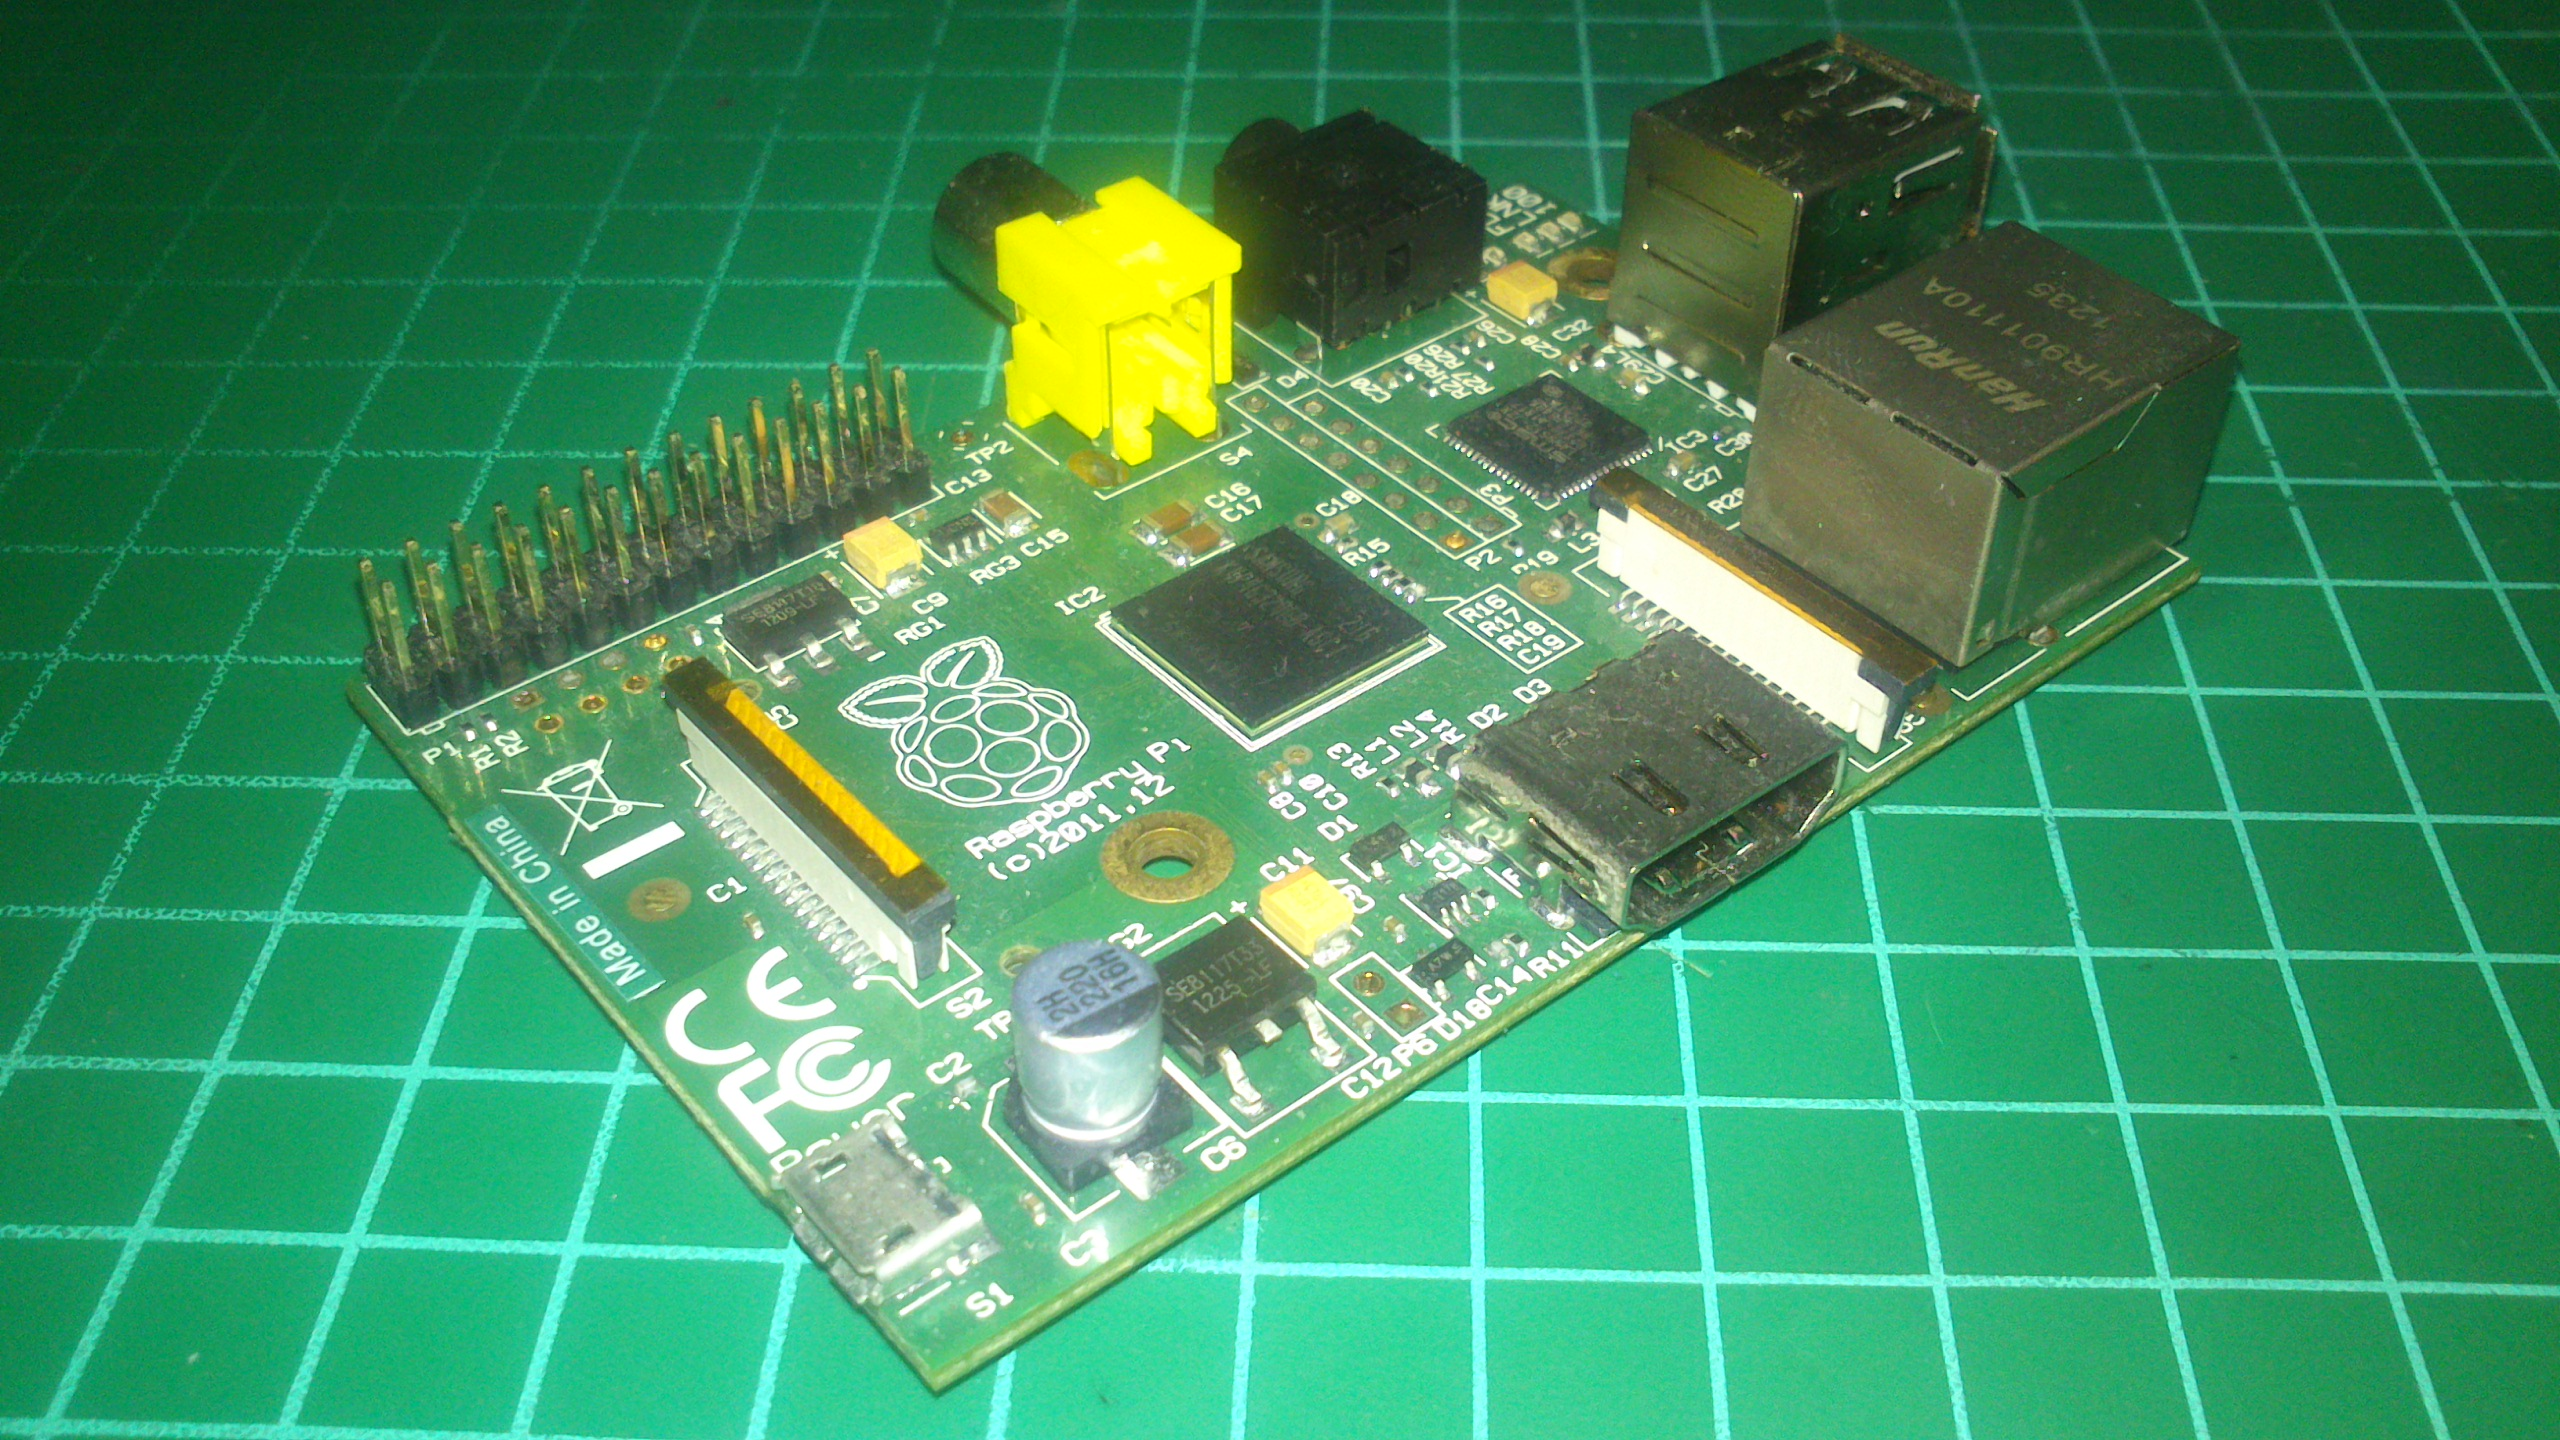
\includegraphics[scale=0.06]{images/RPi.jpg}
\caption{Raspberry Pi a utilitzar}
\label{RPiImage}
\end{center}
\end{figure}
%\end{tabular}

S'ha optat per aquesta opció pel seu econòmic preu, la velocitat de processament i baix consum. A més, s'ha volgut ampliar els coneixements d'aquest petit monstre. En particular s'utilitza la segona revisió del model B:

\begin{figure}[h!]
\begin{center}
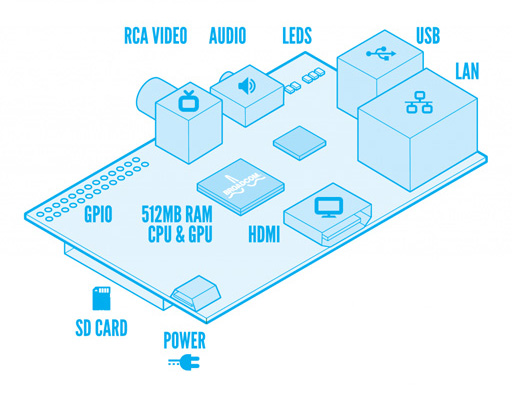
\includegraphics[scale=0.3]{images/RPi2.jpg}
\caption{Conectors de la Raspberry Pi}
\label{RPiConn}
\end{center}
\end{figure}

%\begin{tabular}{cc}
%\hspace{1cm}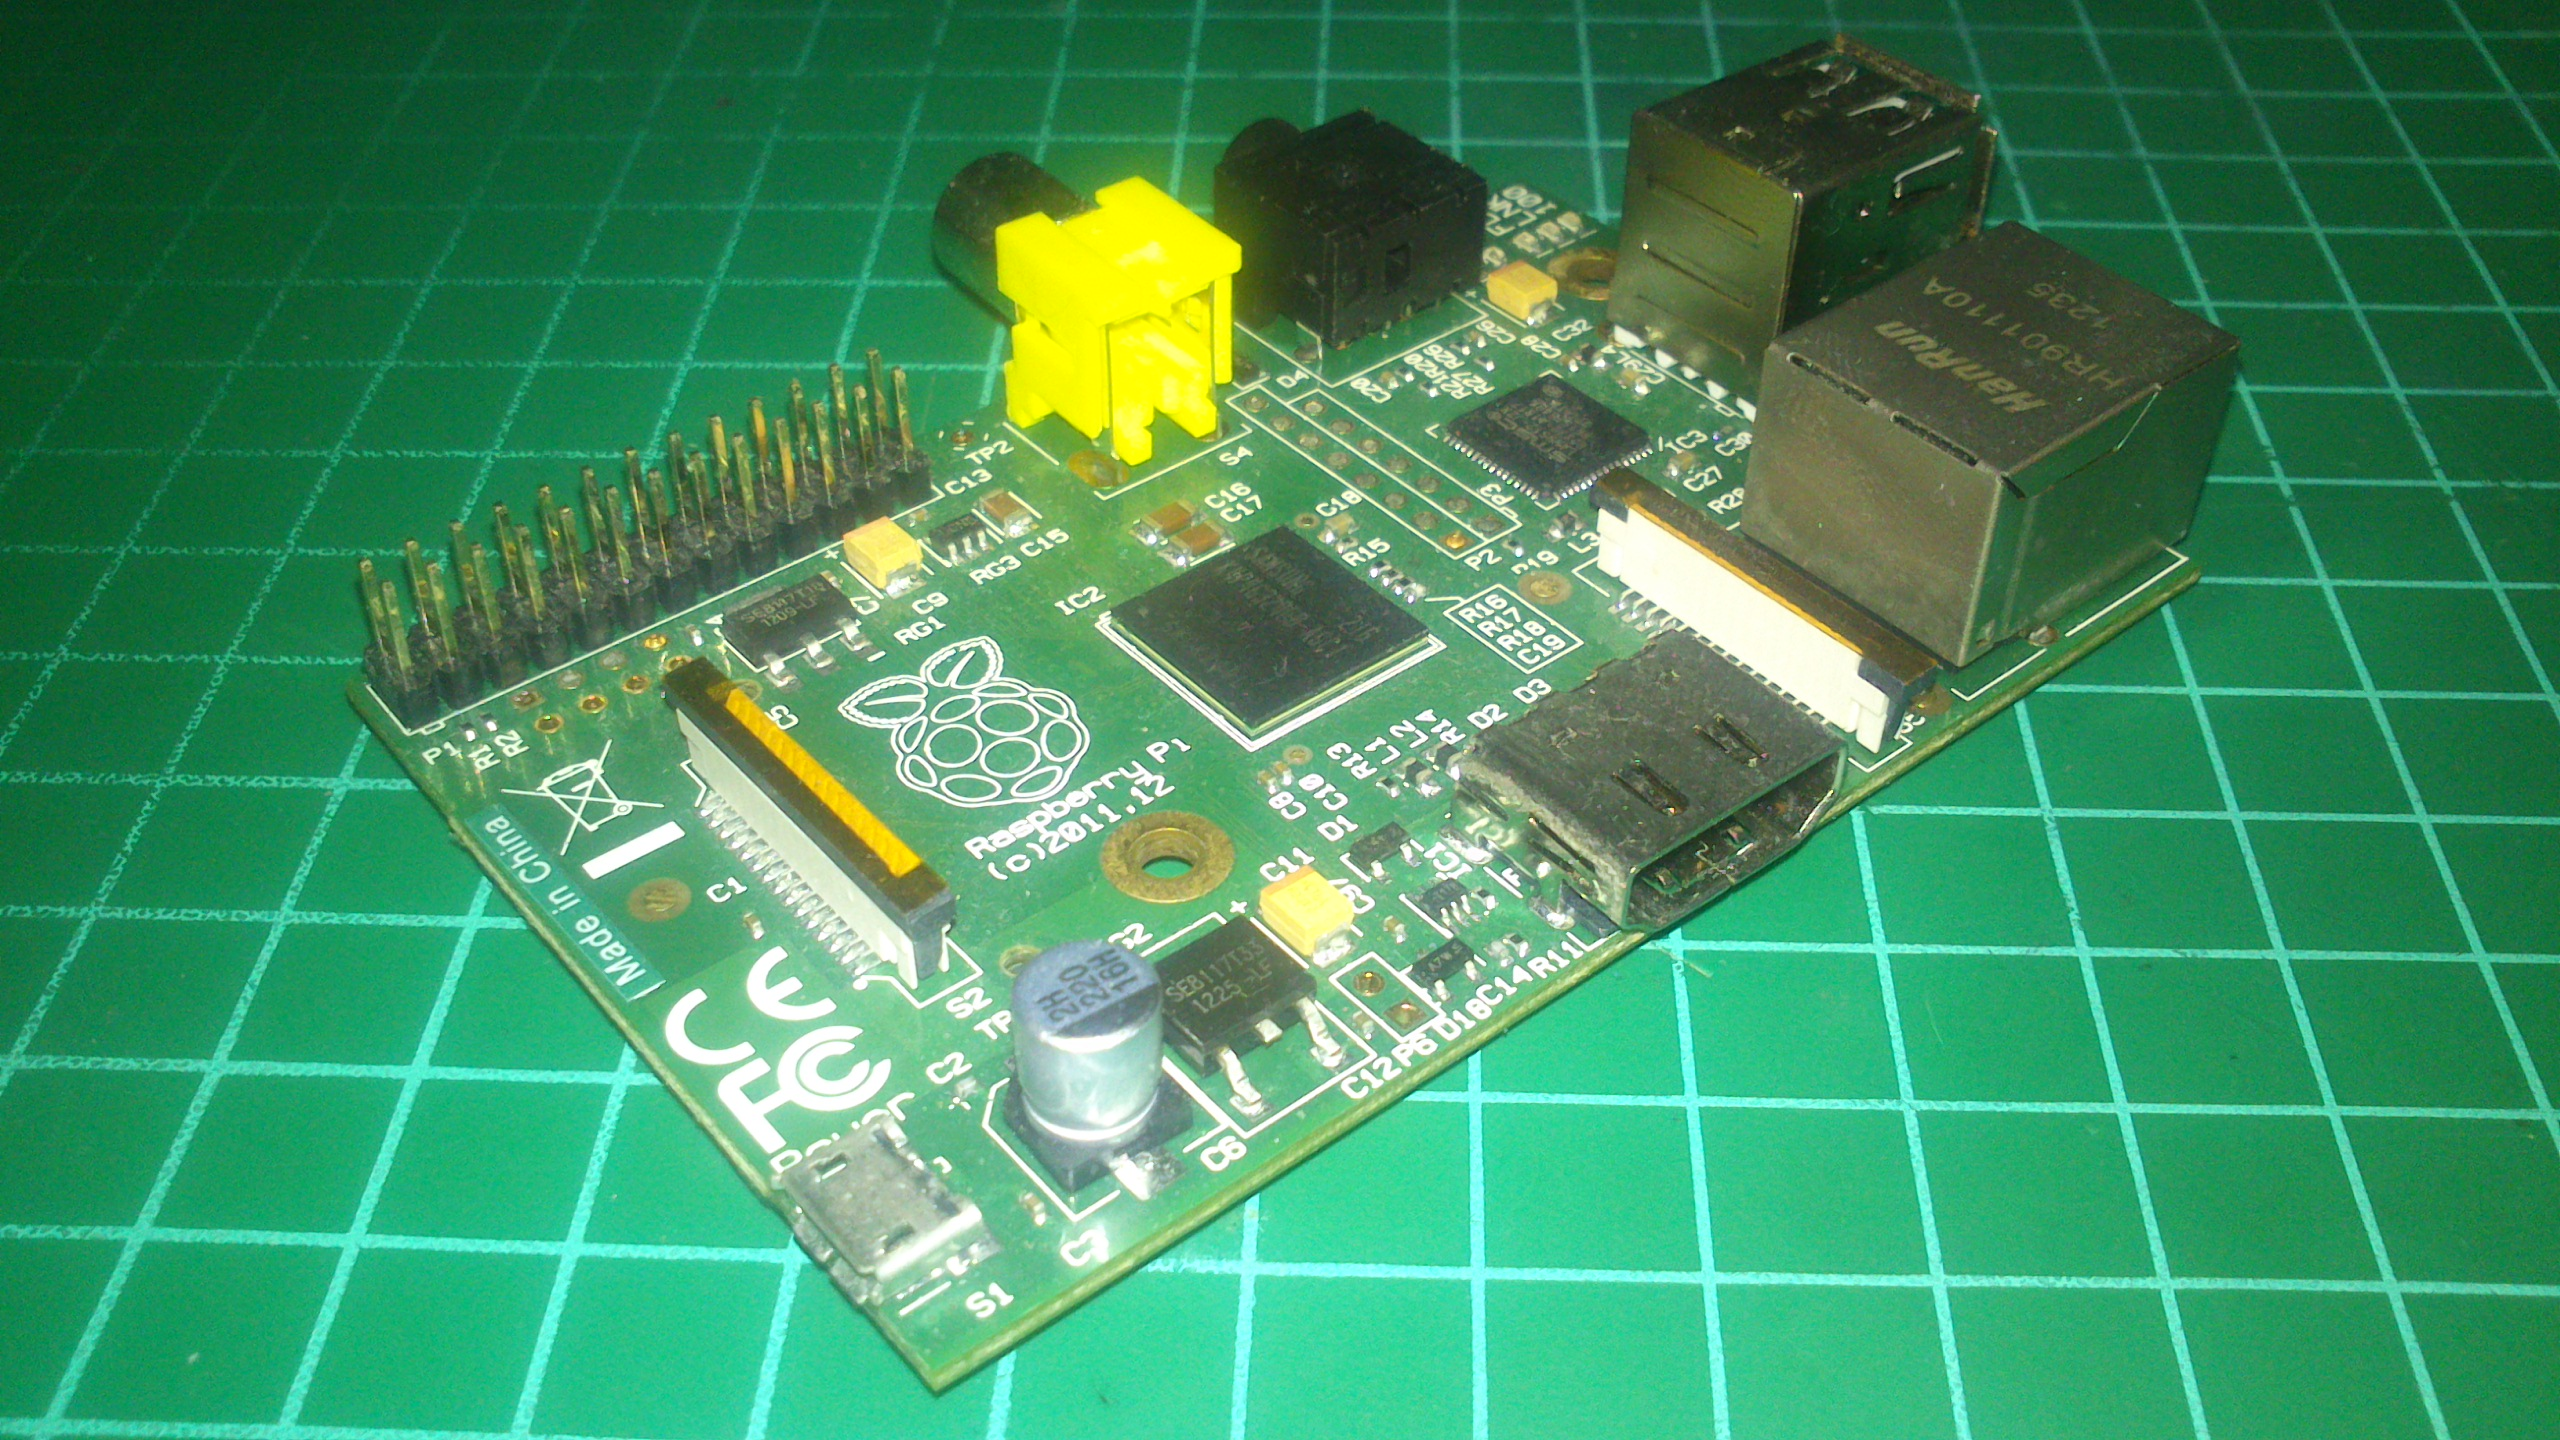
\includegraphics[scale=0.06]{images/RPi.jpg}
%& \hspace{0.5cm} 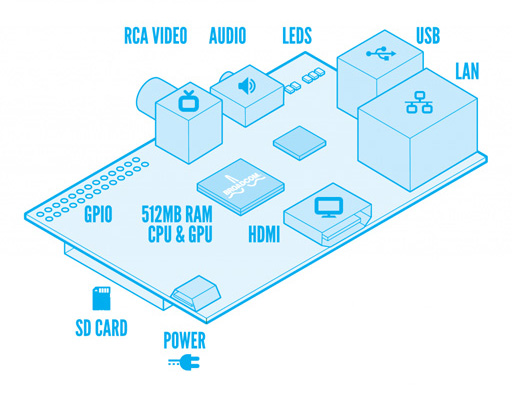
\includegraphics[scale=0.3]{images/RPi2.jpg}
%\end{tabular} \\

Té un System-on-Chip (SoC) Broadcom BCM2835 amb un ARM1176JZF-S a 700 Mhz, una GPU VideoCore IV i 512 MB de memòria RAM. Disposa de dos ports USB, una sortida mini-jack 3.5mm, sortida d'audio/vídeo HDMI, una sortida RCA i un port RJ45 10/100 d'Ethernet. 

L'alimentació es realitza per mitjà d'un mini USB a 5V/700mA, amb un consum de 3.5W. El sistema operatiu és un Raspbian, gravat en una targeta SD de 4GB. Disposa d'un conjunt de pins que permeten comunicació amb perifèrics de baix nivell UART, I2C, SPI i 8 pins de propòsit general (General Porpouse Input Output o GPIO).

\subsubsection*{GY-521 MPU-6050}
Es tracta d'una Unitat de Mesura Inercial (IMU en anglès) que integra en un mateix encapsulat de $4x4x0.9mm$ un acceleròmetre i un giròscop, ambdós de 3 eixos. Disposa dun conversor ADC de 16 bits per a cada eix i es comunica mitjançant un protocol de comunicació $I2C$. S'ha optat per utilitzar aquest dispositiu pel seu baix cost i la fàcil comunicació que comporta amb la RPi.
\begin{figure}[h!]
\begin{center}
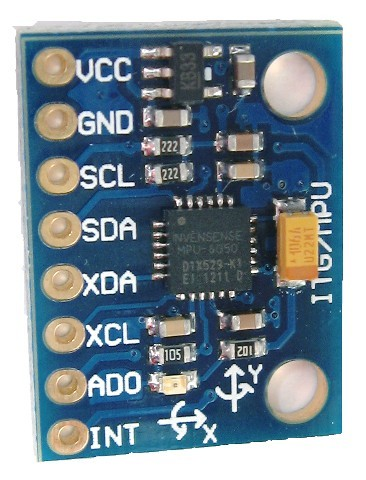
\includegraphics[scale=0.12]{images/mpu-6050.jpg} 
\caption{IMU MPU-6050}
\end{center}
\end{figure}\\
Com a característiques dels sensors: el giròscop té un rang de  $\pm250,\pm500,\pm1000,\pm2000$ graus/segon, i l'accel·leròmetre de $\pm2g,\pm4g,\pm8g,16g$. La tensió d'alimentació és del rang de $2.375V-3.46V$ i cap la possibilitat d'utilitzar un mòdul $DMP$ (Digital Motion Processor), però s'ha decidit implementar un filtre de Kalman per llegint les dades en cru (raw) de la cua $FIFO$ del sensor.

\subsubsection*{Emissor-Receptor}
Amb aquest parell de components es transmet la consigna generada des del transmissor cap al receptor mitjançant ones de radio. El model que s'utilitza és el $Turnigy 5X 5Ch Mini$, per què és un model fàcil d'utilitzar i econòmic. Les especificacions tècniques més rellevants són: 

\begin{figure}[h!]
\begin{center}
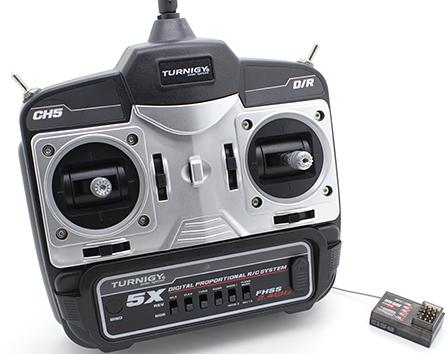
\includegraphics[scale=0.4]{images/E_R.jpg} 
\caption{Emissora i Receptor}
\end{center}
\end{figure}

El transmissor té unes dimensions de $156x152x50mm$, un pes de 265g i s'alimenta a 6V (4 bateries AA). El receptor té unes mides de $33.5x20.5x13mm$ i s'alimenta a 4.8-6V. Disposa de 5 canals de radio, amb transmissió segura a 2.4GHz amb el mètode FHSS. Pot configurarse per traballar amb dos modes (mode1-mode2).

La senyal que es reb per cada canal en el receptor és de $PWM$ de $50Hz$ amb un Duty que veria de $1ms$ a $2ms$.

%% Especificación por canal de los PWM: mínimo y máximo Duty
%% Mirar con osciloscopio la señal

\subsubsection*{Bateria LiPo}
Per a alimentar a tot el conjunt s'utilitza una LiPo $Turnigy 2200mAh 3S1P 25C$. Per tant, és capaç d'entregar 2.2A durant una hora, i com que la capacitat és de 25C, la descàrrega pot ser de $2.2*25=55A$ amb un pic de descàrrega de 35C, és a dir, amb un pic de $2.2*35=77A$ durant 10 segons. Aquesta bateria està formada per tres cel·les que proporcionen un voltatge total d'uns $11.1V$:\\
\begin{center}
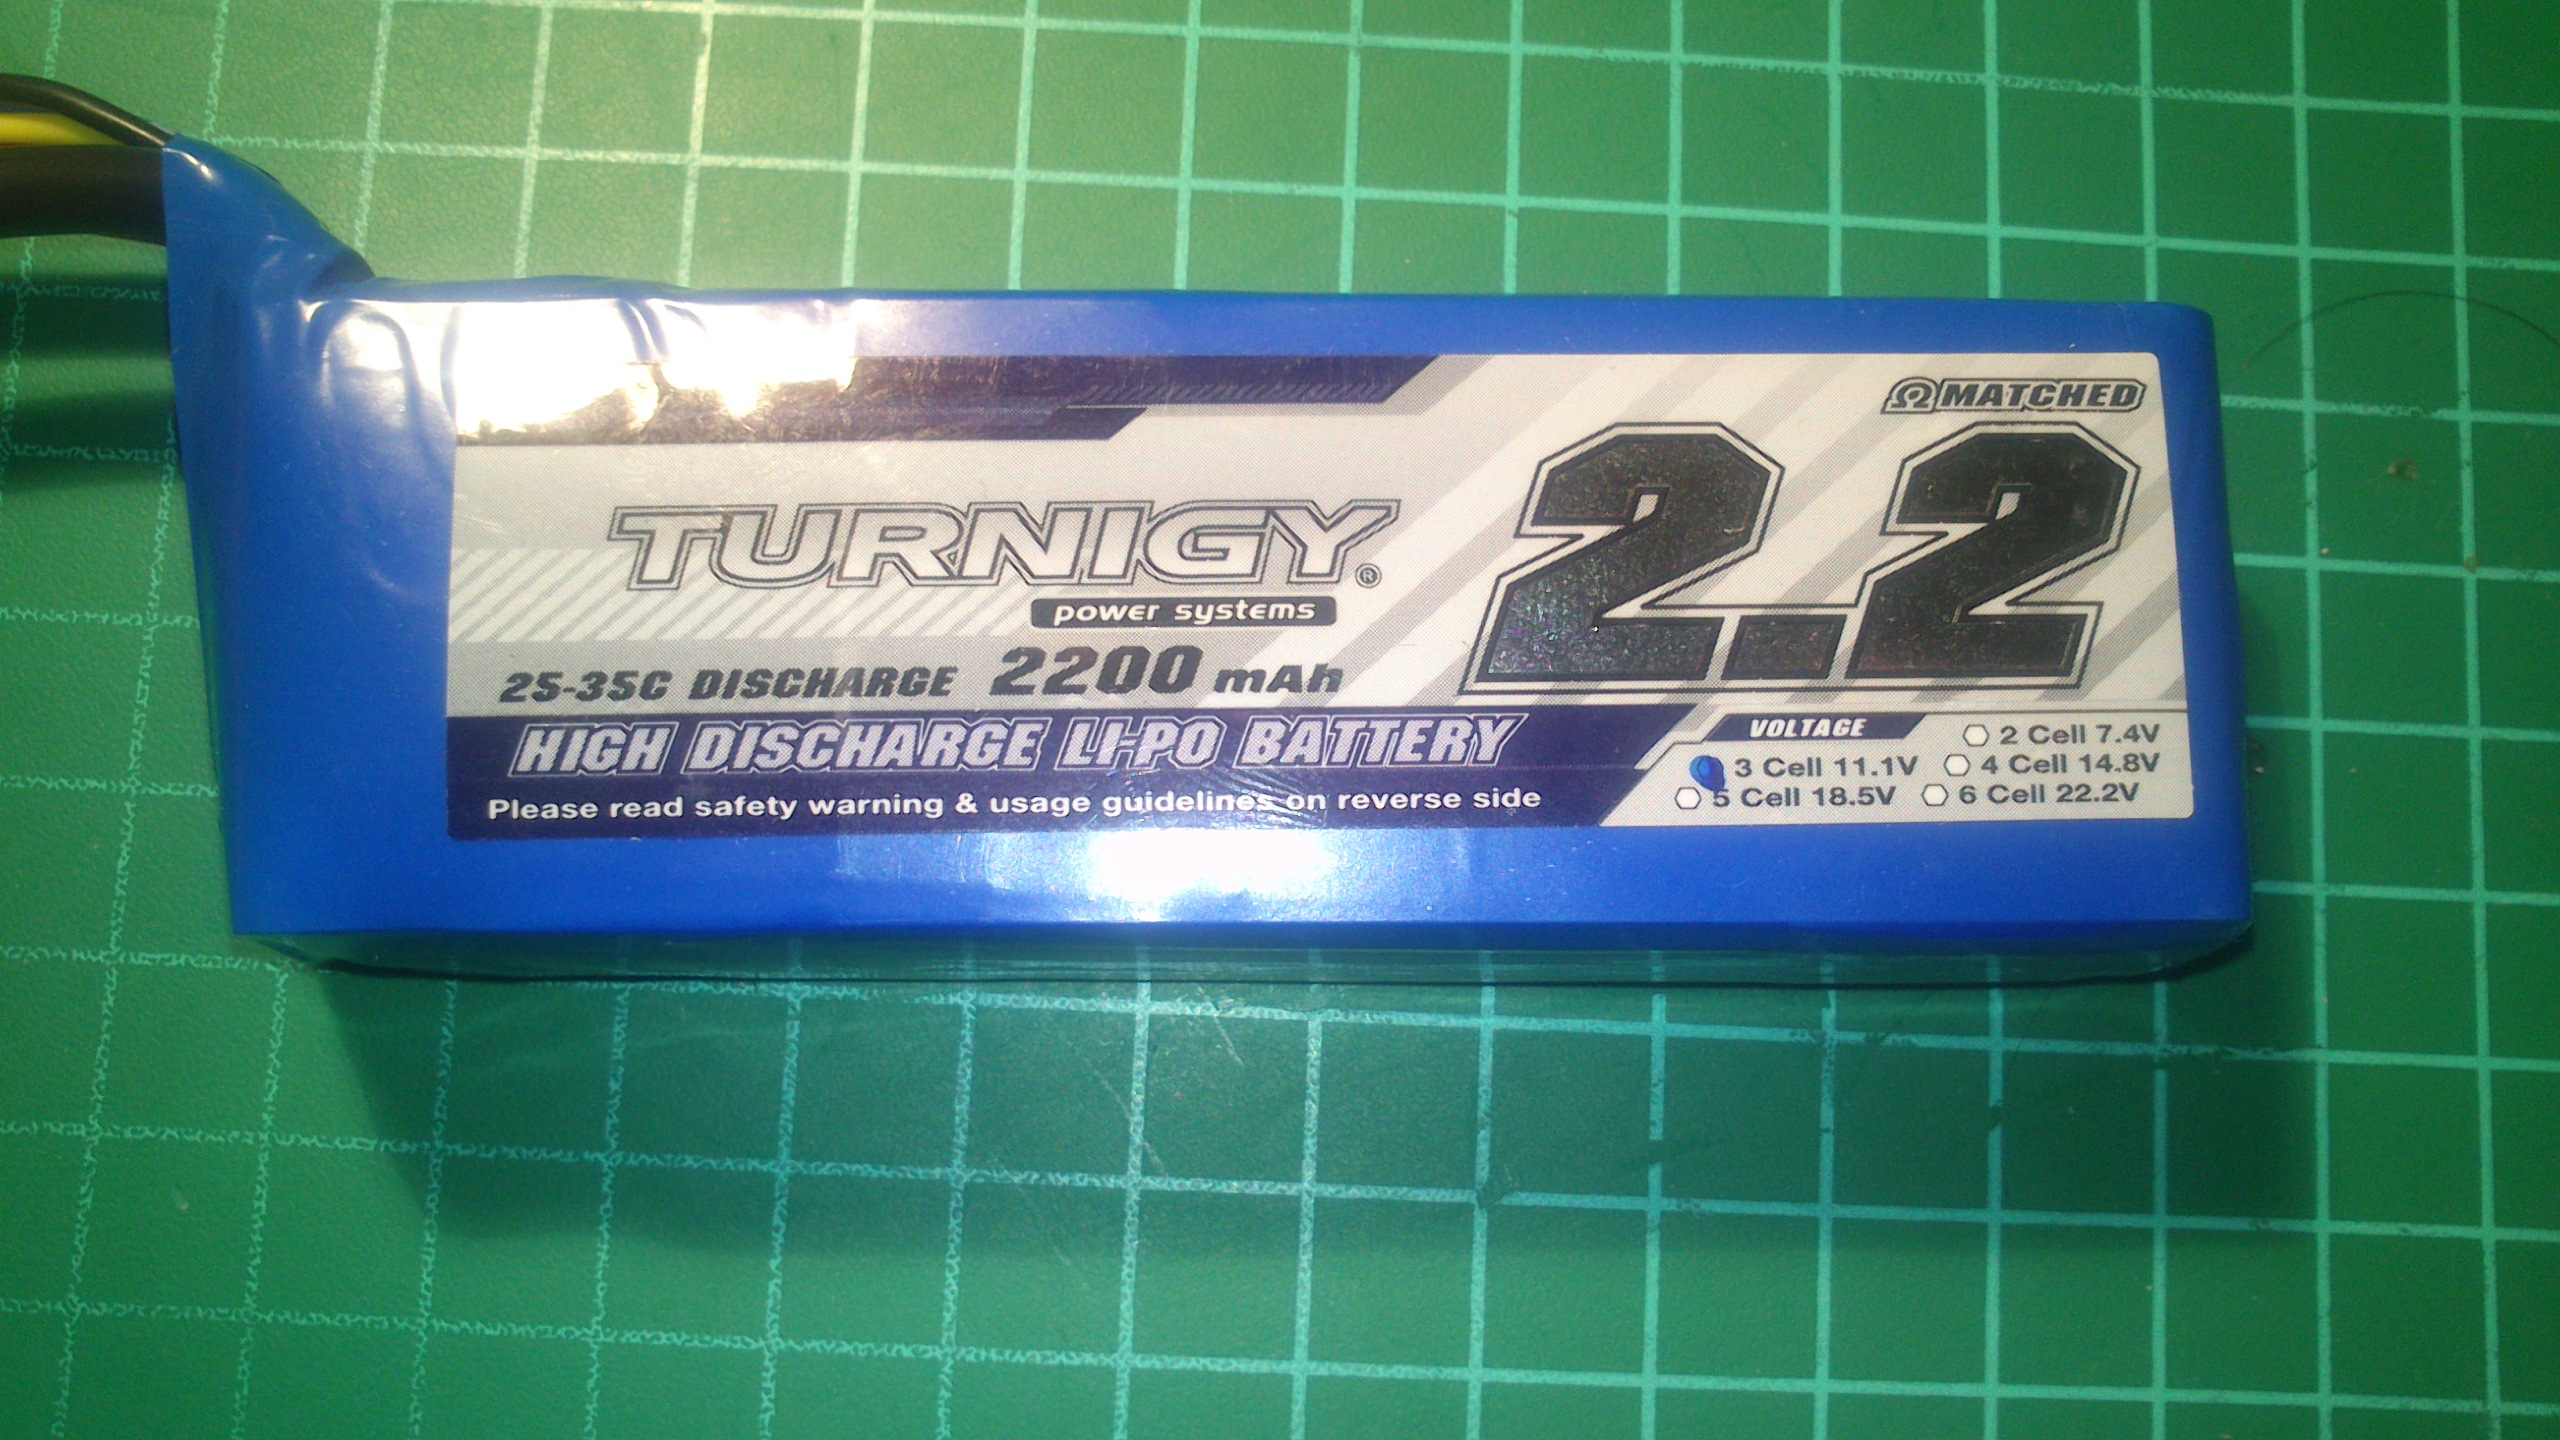
\includegraphics[scale=0.1,viewport=0 400 2560 1250,clip]{images/LiPo.jpg} \\
\end{center}
El conector de càrrega és el $JST-XH$ i el de descàrrega el $XT60$. Per a tenir en compte amb per al quadcopter és interessant saber que pesa $188g$ i respecte a l'estructura (frame) que les seves dimensions són de $105x33x24mm$.

\subsubsection*{Regulador Step-Down}
Per adaptar la tensió de 11.1V de la bateria LiPo a 5V per alimentar la Raspberry Pi, és necessari un regulador. En aquest cas es té l'Interruptor-Mode Màxim BEC LM2576S, que proporciona fins a 3A de corrent \\
\begin{center}
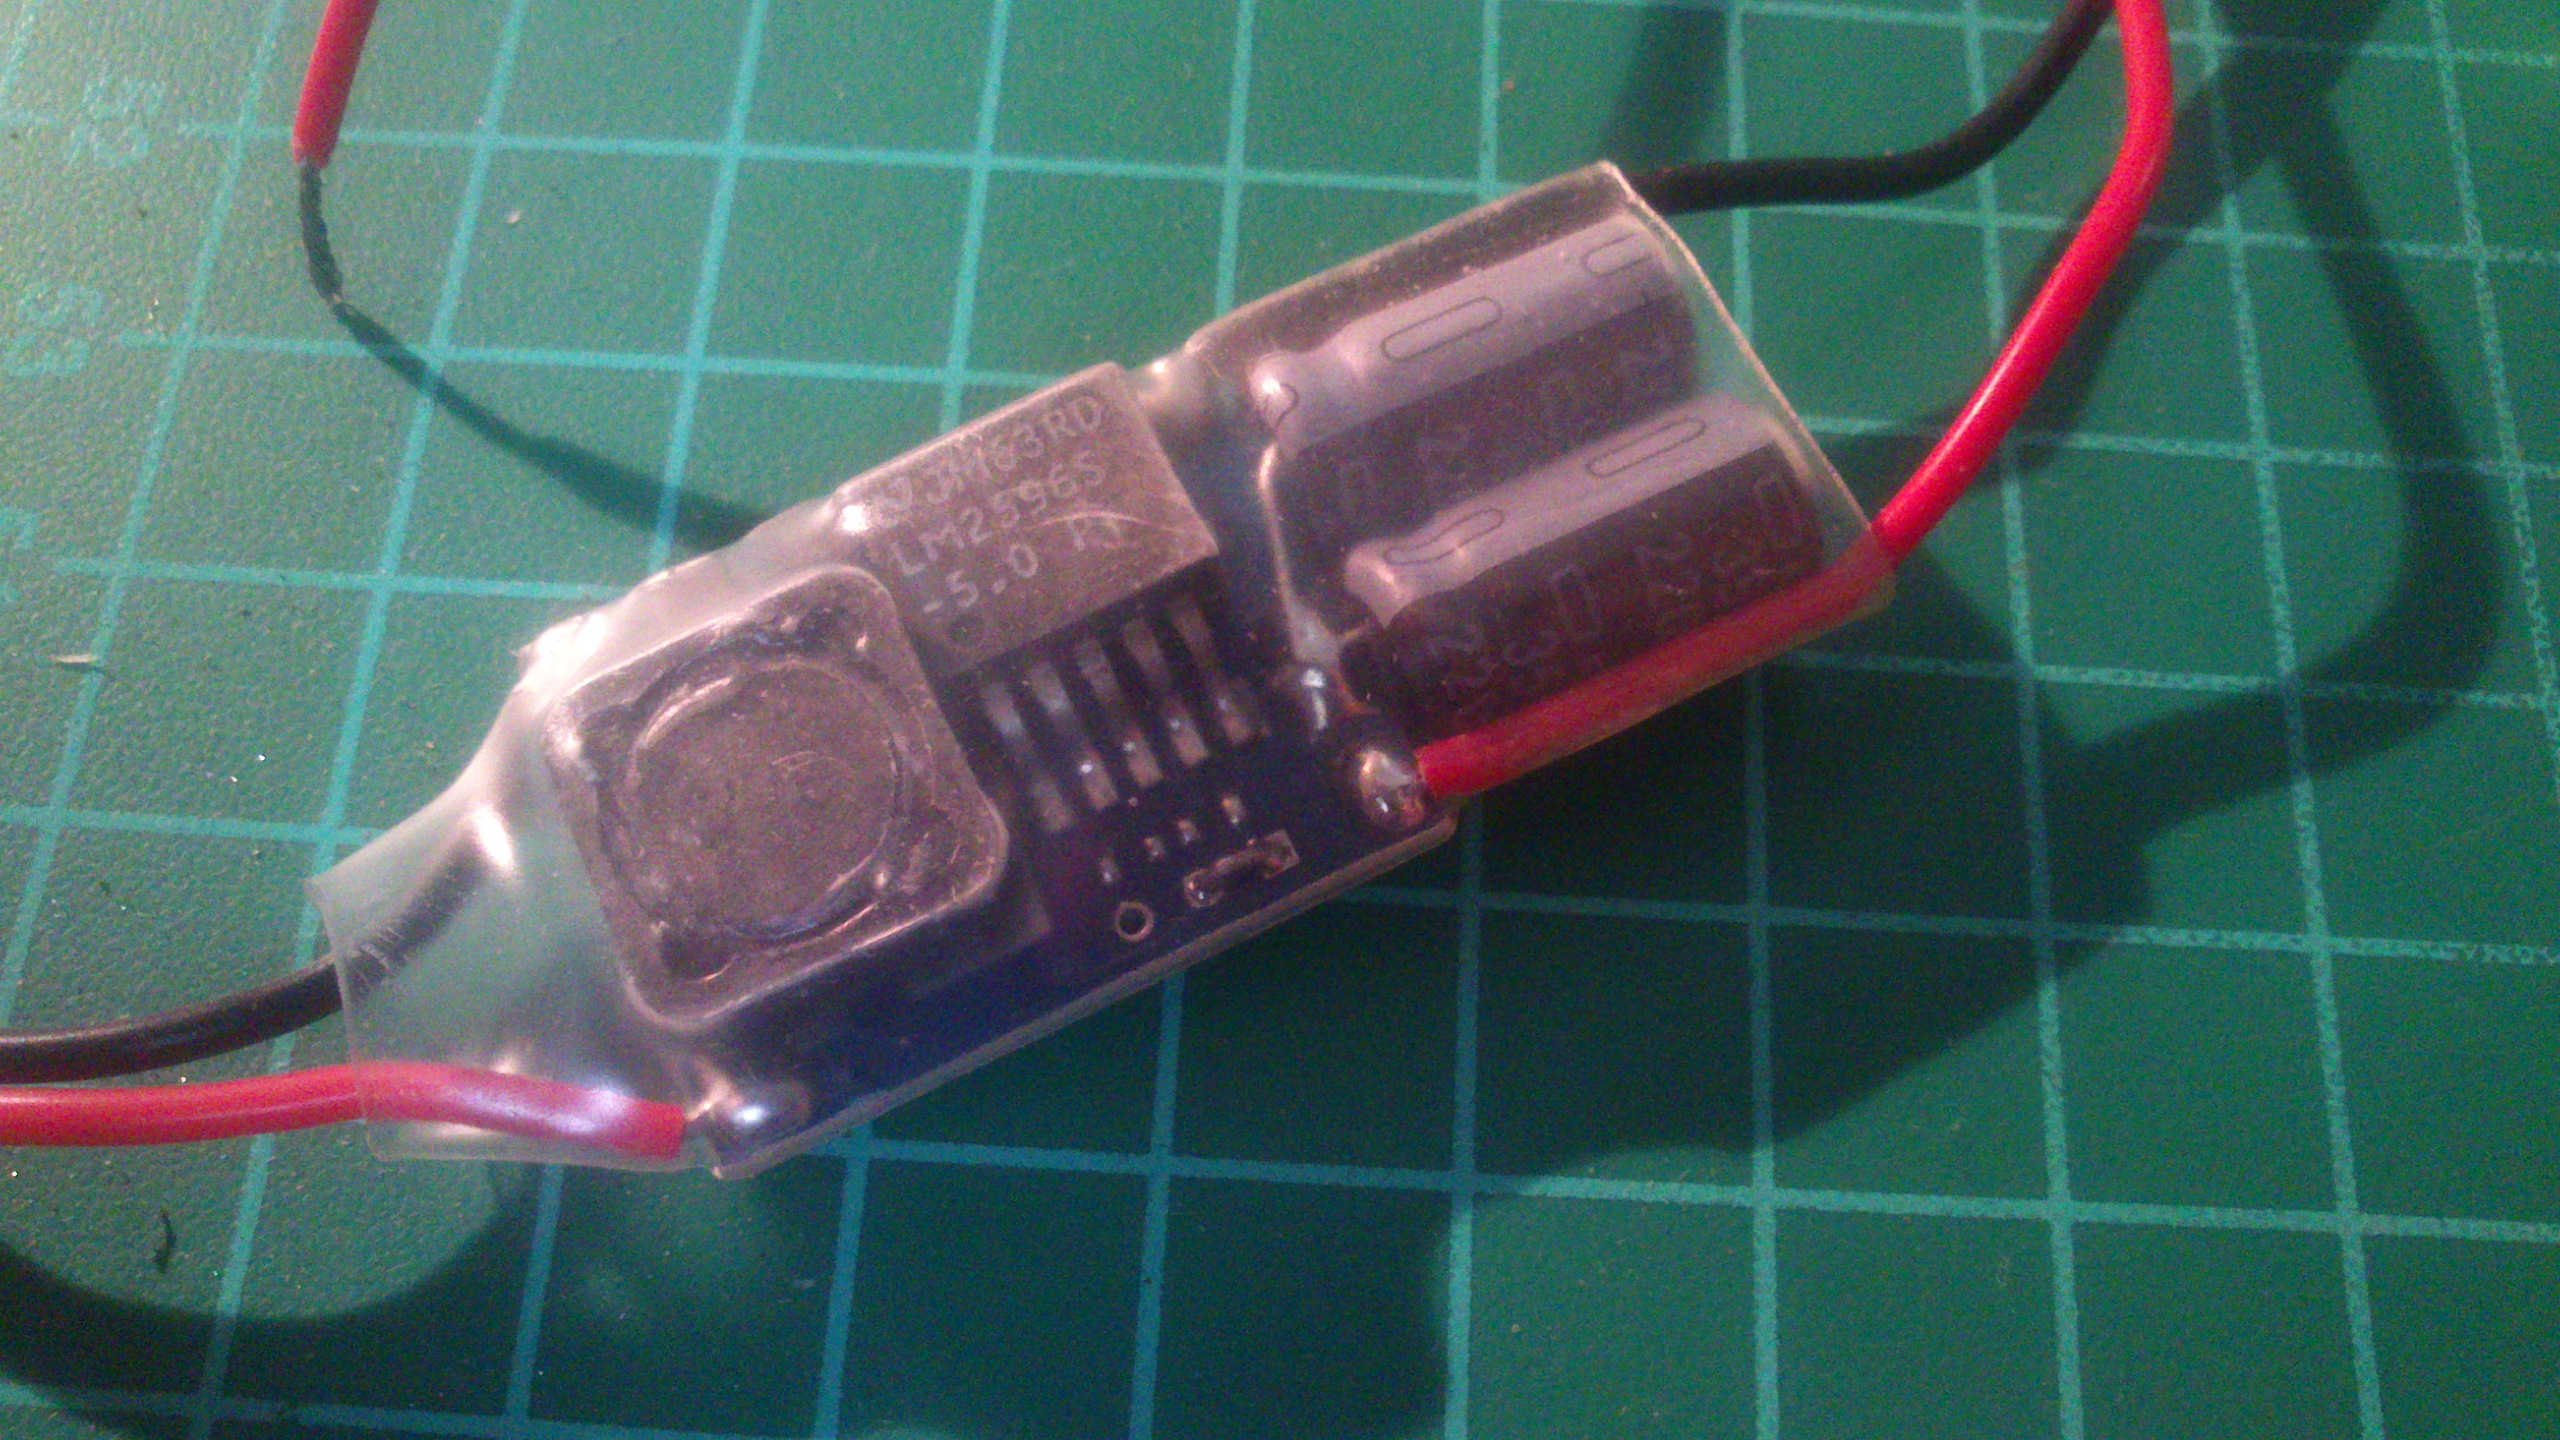
\includegraphics[scale=0.06]{images/Reg_stepdown.jpg}
\end{center}

L'esquema del component \cite{lm2576s}:

\begin{center}
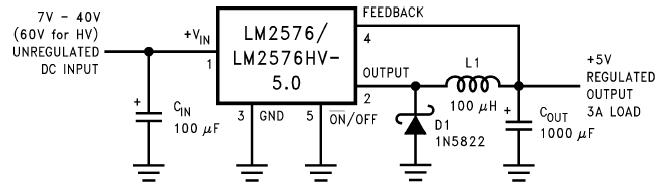
\includegraphics[scale=0.55]{images/lm2576s.jpeg} 
\end{center}

\subsubsection*{Motors Brushless}
Els actuadors que s'utilitzen són motors brushless (BL-DC). En partircular el Turnigy 2213 20turn 1050kv 19A Outrunner.
Es tracta de màquines síncrones d'imans permanents, en comptes d'utilitzar electroimants, on el camp magnètic està uniformement repartit a l'entreferro. S'anomenen també de força electromotriu (FEM) trapezoidal perquè a velocitat constant la FEM té aquesta forma. 
Per a controlarl-lo s'utilitzar un inversor (inverter), la commutació deixa de ser mecànica i per tant l'armadura de la màquina pot ser l'estator. Això permet arribar a voltatges d'ús i velocitats de funcionament més alts.
Les seves especificacions més rellevants són:
\begin{itemize}
\item Kv: 1050rpm/V
\item Corrent de treball: 6A ~ 16A
\item Corrent de pic: 19A
\item Pes: 56g
\item Dimensions: 27.6 x 32mm
\item Mida de l'eix: 3.175mm
\end{itemize}
El primer paràmetre fa referència a quants rpm's funcionarà el motor per Volt aplicat. A aquest valor se li aplica un percentatge $\%NLS$ (Percentatge de Velocitat sense Càrrega, típicament de 70\%) per a quantes revolucions per minut funcionarà:

\begin{equation}
Kv  \cdot V \cdot \%NLS = 1050 \cdot \frac{rpm}{V}\cdot V \cdot 0.70 = 8085 \>\> rpm
\end{equation}

Aquesta velocitat és teòrica, i com que no hi ha un llaç de control sobre aquesta, no es tindrà en compte. En canvi, s'atacarà al motor amb la señal de PWM que s'envia al Variador que el controla. La relació entre la senyal de PWM i la força, així com el consum que es desenvolupa es troben als Annexos. 

\subsubsection*{Variador ESC}

Per a controlar un motor brushless l'etapa de potència a utilitzar es un ESC (Electronic Speed Controller) que és un  variador que consta d'un inversor trifàsic:

\begin{center}
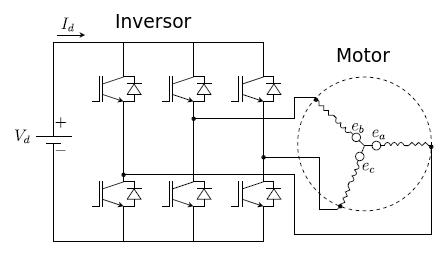
\includegraphics[scale=0.4]{images/ESC.jpeg}
\end{center}

El model a utilitzar és el Turnigy AE-20A Brushless ESC. L'ús d'aquest tipus es justifica amb l'amperatje que suporta, en quant els motors consumeixen com a pic fins a 19A, que és menys del màxim de la corrent d'aquest Variador.

Specification:
Output:  Continuous 20A, burst 25A up to 10 seconds.
Input Voltage:  2-4 cells lithium battery or 5-12 cells NIMH battery.   
BEC:  Linear 2A @ 5V
Control Signal Transmission: Optically coupled system.
Max Speed:     
   2 Pole: 210,000rpm
   6 Pole: 70,000rpm
   12 Pole: 35,000rpm
Size:  50mm (L) * 26mm (W) * 12mm (H).
Weight:  19g.

Features:
High performance microprocessor brings out the best compatibility with all kinds of motors and the highest driving efficiency.
Wide-open heatsink design to get the best heat dissipation effect.
Improved Normal, Soft, Very-Soft start modes, compatible with aircraft and helicopter. 
Smooth, linear, quick and precise throttle response.
Multiple protection features: Low-voltage cut-off protection / Over-heat protection / Throttle signal loss protection
Programable via transmitter
Programming features:
Brake setting (we recommend using brake for only folding props applications)
Battery type(Li-xx or Ni-xx) 
Low voltage cutoff setting 
Factory default setup restore 
Timing settings (to enhance ESC efficiency and smoothness) 
Soft acceleration start ups (for delicate gearbox applications)
Low voltage cutoff type (power reduction orirnmediate shutdown)
 
Factory default settings:
Brake:  off 
Battery type:  Li-xx (Li-ion or Li-Po) 
Low voltage cutoff threshold:  Soft cut-off (2.6V) 
Timing setup:  Low 
Soft Acceleration Start Up:  Normal \\
Low voltage cutoff type:  Medium


\subsubsection*{Frame}
Peso 190g

\subsubsection*{Hèlix}


\newpage
\subsection{Muntatge}
% Descripción del procedimiento por pasos y con fotos

\begin{center}
\begin{tikzpicture}
%%% POWER LINES
\path[draw] (1,8.25) node {\large 12V};
\path[draw] (2,8.25) node {\large 0V};
\path[draw,line width=6pt,color=red,o-o] (1,1) -- (1,8);
\path[draw,line width=6pt,color=black,o-o] (2,1) -- (2,8);

%%% LIPO LEVEL
\path[draw,line width=2pt,color=red] (1,6) -- (3,6);
\path[draw,line width=2pt,color=black] (2,5.5) -- (3,5.5);
\path[draw] (3.8,5.75) node[draw,line width=3pt] (nodeA) {\huge LiPo};
\path[draw] (7.2, 5.75) node[draw,line width=3pt] (nodeA) {\huge IMU};
\path[draw,line width=2pt,color=olive] (7.2,5.35) -- (7.2,4.6);
\path[draw] (7.6,5) node (nodeC) { I2C};
\path[draw] (9.8, 5.75) node[draw,line width=3pt] (nodeA) {\huge Rec.};
\path[draw, line width=2pt,color=green] (9.8, 5.34) -- (9.8, 4.5) -- (7.95, 4.5);
\path[draw] (9, 4.8) node {5xCHNL};
\path[draw,line width=2pt,dotted, color=cyan](10.6,5.75) -- (12.3,5.75);
\path[draw] (13, 5.75) node[draw,line width=3pt] (nodeA) {\huge Em.};

%%% BUCK LEVEL
\path[draw,line width=2pt,color=red] (1,4.5) -- (3,4.5);
\path[draw,line width=2pt,color=black] (2,4) -- (3,4);
\path[draw] (4.1,4.25) node[draw,line width=3pt] (nodeA) {\huge BUCK};
\path[draw,line width=2pt,color=red] (5.26,4.5) -- (6.5,4.5);
\path[draw,line width=2pt,color=black] (5.2,4) -- (6.5,4);
\path[draw] (7.2,4.25) node[draw,line width=3pt] (nodeA) {\huge RPi};
\path[draw] (5.8,4.8) node (nodeC) {5V};
\path[draw, line width=2pt, color=green] (7.95,4)--(9.8,4) -- (9.8,3.2);
\path[draw] (9.2,3.65) node {PWM};

%%% ESC LEVEL
\path[draw, line width=2pt, color=red] (1,3) -- (9,3);
\path[draw, line width=2pt, color=black] (2,2.5) -- (9,2.5);
\path[draw] (9.8,2.75) node[draw,line width=3pt] (nodeC) {\huge ESC};
\path[draw] (10.3,2.1) node (nodeC) {\large (x4)};
\path[draw, line width=2pt, color=blue] (10.6,3) -- (12,3);
\path[draw, line width=2pt, color=blue] (10.6,2.75) -- (12,2.75);
\path[draw, line width=2pt, color=blue] (10.6,2.5) -- (12,2.5);
\path[draw] (13,2.75) node[draw,line width=3pt] (nodeC) {\huge Motor};
\path[draw] (13.7,2.1) node (nodeC) {\large (x4)};
\end{tikzpicture}
\end{center}

% Descripcion general de como se genera, envia y procesa la consigna
% Imagen con esquema
% Explicar que la App es en java y para Android y que envia la informacion a la RPi (configurada como AccessPoint).
% Dar el codigo de la aplicacion

\newpage
\section{Anàlisi econòmic} \label{economics}
\newpage

\section{Estudi d'impacte ambiental} \label{impacto}
\newpage

\section{Conclusiones} \label{conclusiones}
\subsection*{Futuras aplicaciones}
\newpage

\begin{thebibliography}{99}
\bibitem{QuadPaper} Teppo Luukkonen (August 22,2011). \textit{Modelling and control of quadcopter}
\bibitem{RPiWiki} Wikipedia de la Raspberry Pi: \url{http://en.wikipedia.org/wiki/Raspberry_Pi}
\bibitem{IMUArduino} Accel·leròmetre i Giròscop MPU-6050 per a Arduino: \url{http://playground.arduino.cc/Main/MPU-6050#.UzhsVCK9jb4}
\bibitem{6050Esp} MPU-6050. Especificació del producte: \url{http://www.invensense.com/mems/gyro/documents/PS-MPU-6000A-00v3.4.pdf}
\bibitem{6050RegMap} MPU-6050. Mapa de Registres i descripcions: \url{http://www.invensense.com/mems/gyro/documents/RM-MPU-6000A-00v4.2.pdf}
\bibitem{lm2576s} LM2576S Datasheet: \url{http://www.ti.com/lit/ds/symlink/lm2576.pdf}
\bibitem{wiringPi} Llibrería wiringPi: \url{http://wiringpi.com/}
\end{thebibliography}{}
\newpage

\section*{Agraïments}
\newpage

\section*{ANNEXES}
\subsection*{Annex 1: Obtenció vector de forces}
Per a treballar amb la dinàmica del sistema s'obté el vector de forces a partir del Lagrangià:
\begin{verbatim}
clear all
clc

%%% Para usar la funcion Laplace en el archivo Laplace.m se deben declarar
%%% las variables de esta manera:

syms x dx ddx y dy ddy z dz ddz Phi dPhi ddPhi Theta dTheta ddTheta Psi dPsi ddPsi
syms f1 f2 f3 f4 m1 m2 m3 m4
% syms w1 w2 w3 w4
syms Ixx Iyy Izz
syms Ax Ay Az               % No se tienen en cuenta coeficientes de friccion
syms k m g l b

l=0.165             % longitud de los brazos
Ixx=0.004           % Momento de inercia del eje x 
Iyy=0.004           % Momento de Inercia del eje y
Izz=0.008           % Momento de Inercia del eje z
m=0.85              % Peso del Quadcopter
g=9.81              % gravedad 

%%% El vector de variables que se usaran

v=[x dx ddx y dy ddy z dz ddz Phi dPhi ddPhi Theta dTheta ddTheta Psi dPsi ddPsi]

Xi=[x; y; z]
dXi=[dx; dy; dz]

Eta=[Phi; Theta; Psi]
dEta=[dPhi; dTheta; dPsi]

Q=[Xi; Eta]
dQ=[dXi; dEta]

II=[[Ixx 0 0];
    [0 Iyy 0];
    [0 0 Izz]]

A=[[Ax 0 0];
   [0 Ay 0];
   [0 0 Az]]   
   
R=[[cos(Psi)*cos(Theta) cos(Psi)*sin(Theta)*sin(Phi)-sin(Psi)*cos(Phi) cos(Psi)*sin(Theta)*cos(Phi)+sin(Psi)*sin(Phi)];
    [sin(Psi)*cos(Theta) sin(Psi)*sin(Theta)*sin(Phi)+cos(Psi)*cos(Phi) sin(Psi)*sin(Theta)*cos(Phi)-cos(Psi)*sin(Phi)];
    [-sin(Theta) cos(Theta)*sin(Phi) cos(Theta)*cos(Phi)]]

Weta=[[1 0 -sin(Theta)];
      [0 cos(Phi) cos(Theta)*sin(Phi)];
      [0 -sin(Phi) cos(Theta)*cos(Phi)]]
  
J=transpose(Weta)*II*Weta  
  
L=m/2*transpose(dXi)*dXi+(1/2)*transpose(dEta)*transpose(Weta)*II*Weta*dEta-m*g*z

%%% Aqui se obtiene con el Lagrangiano el vector de fuerzas F segun
%%% F=(d/dt)(dp(L)/dp(dq))-d(L)/dq

F=Lagrange(L,v)

%%% Derivando a mano se obtiene que TauB=J*ddEta+CdEta 
%%% Y como TauB=[F(4); F(5); F(6)], se tiene que el termino de Coriolis es:

CdEta=[F(4); F(5); F(6)]-J*[ddPhi; ddTheta; ddPsi]

%%% Hasta se tiene el producto Coriolis(Eta,dEta)*dEta. Pero como matlab
%%% no elimina las aceleraciones se hace a mano, y queda:

CdEta = [(Iyy*dTheta^2*sin(2*Phi))/2 - (Izz*dTheta^2*sin(2*Phi))/2 - Ixx*dPsi*dTheta*cos(Theta) - (Iyy*dPsi^2*sin(2*Phi)*cos(Theta)^2)/2 + (Izz*dPsi^2*sin(2*Phi)*cos(Theta)^2)/2 - Iyy*dPsi*dTheta*cos(2*Phi)*cos(Theta) + Izz*dPsi*dTheta*cos(2*Phi)*cos(Theta);
          dPhi*(Ixx*dPsi*cos(Theta) - 2*Iyy*dTheta*cos(Phi)*sin(Phi) + 2*Izz*dTheta*cos(Phi)*sin(Phi) + Iyy*dPsi*cos(Phi)^2*cos(Theta) - Izz*dPsi*cos(Phi)^2*cos(Theta) - Iyy*dPsi*cos(Theta)*sin(Phi)^2 + Izz*dPsi*cos(Theta)*sin(Phi)^2)  - Ixx*dPsi^2*cos(Theta)*sin(Theta) + Iyy*dPsi^2*cos(Theta)*sin(Phi)^2*sin(Theta)  + Izz*dPsi^2*cos(Phi)^2*cos(Theta)*sin(Theta);
          -dPhi*(Ixx*dTheta*cos(Theta) - Iyy*dTheta*cos(Phi)^2*cos(Theta) + Izz*dTheta*cos(Phi)^2*cos(Theta) + Iyy*dTheta*cos(Theta)*sin(Phi)^2 - Izz*dTheta*cos(Theta)*sin(Phi)^2 - 2*Iyy*dPsi*cos(Phi)*cos(Theta)^2*sin(Phi) + 2*Izz*dPsi*cos(Phi)*cos(Theta)^2*sin(Phi)) - Iyy*dTheta^2*cos(Phi)*sin(Phi)*sin(Theta) + Izz*dTheta^2*cos(Phi)*sin(Phi)*sin(Theta) + 2*Ixx*dPsi*dTheta*cos(Theta)*sin(Theta) - 2*Izz*dPsi*dTheta*cos(Phi)^2*cos(Theta)*sin(Theta) - 2*Iyy*dPsi*dTheta*cos(Theta)*sin(Phi)^2*sin(Theta)]
      
T=f1+f2+f3+f4               % Fuerza total (Total Thrust)
TB=[0; 0; T]                % Thrust en la referencia del Quadctopter
TauB=[l*(f4-f2);
      l*(f3-f1);
      % (m1+m2+m3+m4)]
      b*(f1-f2+f3-f4)]
\end{verbatim}
\newpage

%\begin{lstlisting}

%\end{lstlisting}

\subsection*{Annex 2:Preparació de la Raspberry Pi}
Per a posar a punt la RPi s'ha d'instal·lar Raspbian i configurar-lo per tal que es pugui comunicar amb la placa MPU-6050.
\subsubsection*{Instalació Raspbian}
Havent introduït la targeta SD en un lector adeqüat, es detecta en una terminal mitjançant l'ordre \textit{df -h}. Suposant que hagués estat gravada anteriorment:
\begin{center}
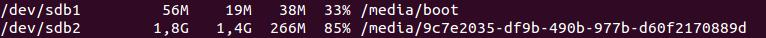
\includegraphics[scale=0.7]{images/InstalRasp1.jpeg}
\end{center}
S'han de desmontar les dos particions, tant la \textit{/dev/sdb1} com la \textit{/dev/sdb2}:
\begin{verbatim}
           umount /dev/sdb1
           umount /dev/sdb2
\end{verbatim}
Havent descarregat la imatge a instalar per exemple a l'Escriptori, es procedeix amb:
\begin{verbatim}
    sudo dd bs=4M if=~/Escritorio/2013-07-26-wheezy-raspbian.img of=/dev/sdb
\end{verbatim}
Passats uns minuts ja es té la SD grabada amb el sistema operatiu Raspbian.
\subsubsection*{Configuració de la Raspberry}
Per tal de poder comunicar la RPi amb la IMU MPU-6050 per I2C és necessari configurar el sistema. Primer és necessari instal·lar els drivers més rellevants. De l'arxiu
\begin{verbatim}
           sudo nano /etc/modules
\end{verbatim}
s'han d'afegir les següents dues línies al final de l'arxiu:
\begin{verbatim}
           i2c-bcm2708
           i2c-dev
\end{verbatim}
En l'arxiu blacklist:
\begin{verbatim}
           sudo vi /etc/modprobe.d/raspi-blacklist.conf
\end{verbatim}
les següents dues línies han de començar amb un signe \# (de comentari):
\begin{verbatim}
           #blacklist spi-bcm2708
           #blacklist i2c-bcm2708
\end{verbatim}
Per provar de connectar el sensor, és necessari seguir primer el connexionat:

\begin{figure}[h!]
\begin{center}
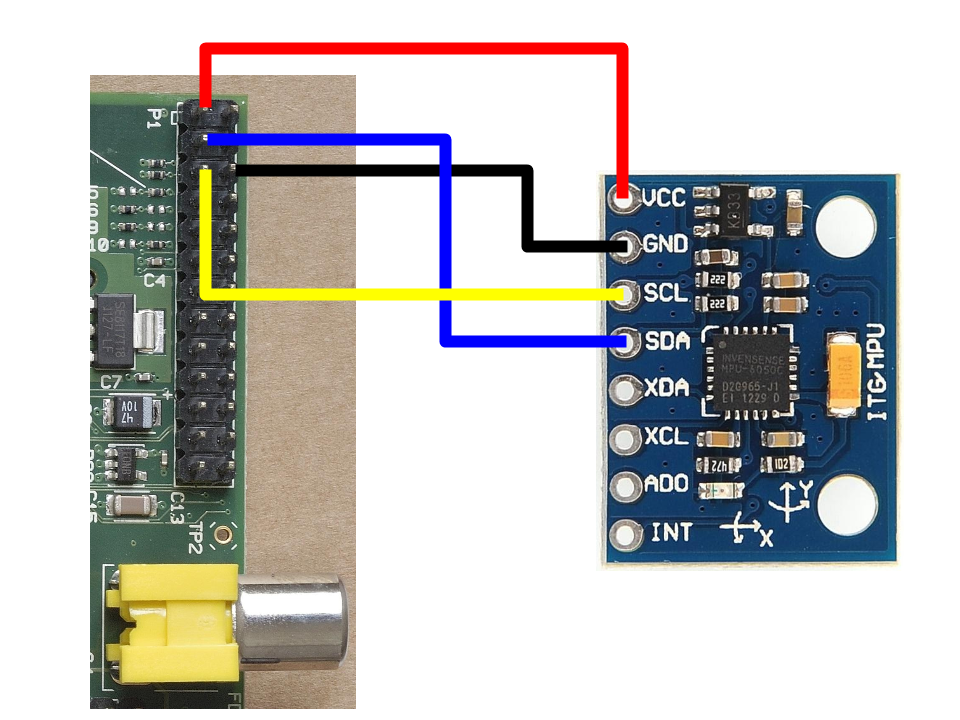
\includegraphics[scale=0.2,viewport=0 200 800 720,clip]{images/ConSens.jpg}
\caption{Connexió per I2C entre MPU-6050 i RPi}
\end{center}
\end{figure}


És a dir:
\begin{itemize}
\item Pin1-3.3V es connecta VCC.
\item Pin3-SDA es connecta a SDA
\item Pin5-SCL es connecta a SCL
\item Pin6-Ground es connecta a GND
\end{itemize} 
S'ha d'instal·lar el paquet $i2c-tools$:
\begin{verbatim}
           sudo apt-get install i2c-tools
\end{verbatim}
Per a veure el sensor s'escriu:
\begin{verbatim}
           sudo i2cdetect -y 1
\end{verbatim}
El resultat és 

\begin{figure}[h!]
\begin{center}
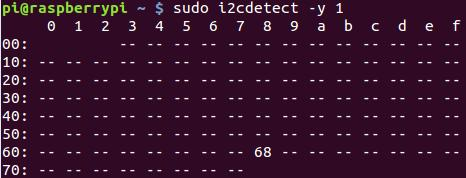
\includegraphics[scale=0.7]{images/i2cdetect.jpg}
\caption{Detecció del sensor MPU-6050}
\end{center}
\end{figure}
que és el dispositiu que correspon al MPU-6050.

\subsubsection*{Llibrería wiringPi}
S'utilitza aquesta llibrería\cite{wiringPi} com a interfície del GPIO (General Porpouse Input Output). Permet, per tant,llegir tant les consignes com els sensors i generar les accions de control. 
La instal·lació i descripció de la llibrería està explicat a la pàgina web incluída a la bibliografía.

\newpage
\subsection*{Annex 3: Filtre de kalman}
\newpage
\subsection*{Annex 4: Caracterització dels motors}
Per tal de poder controlar la planta és necessari saber còm responen els actuadors per tal de realitzar un control precís. D'aquests és necessari saber quina força i moment proporcionen, així com el consum d'energia donat un PWM. 
Per a obtenir una corva de la força respecte del PWM es pesa amb una balança l'acció del motor. La rudimentària bancada que es té per a tal objectiu és d'un colze articulat a un eix de tal manera que la distància de l'eix del motor al fulcre i d'aquest a la balança sigui la mateixa (en aquest cas de 12 cm):

\begin{figure}[h!]
\begin{center}
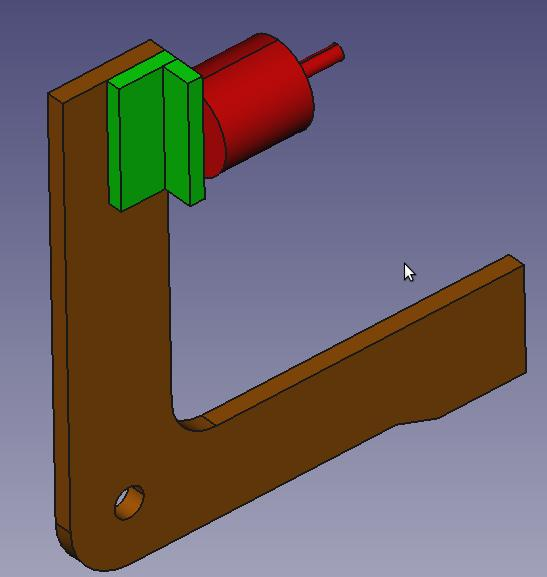
\includegraphics[scale=0.4]{images/bancada1.jpeg}
\caption{Bancada per a l'estudi del motor}
\end{center}
\end{figure}
Les parts estan fetes de fusta (part marró) i plàstic ABS (part verda). Tota l'estructura es subjecta a unes fustes:

\begin{figure}[h!]
\begin{center}
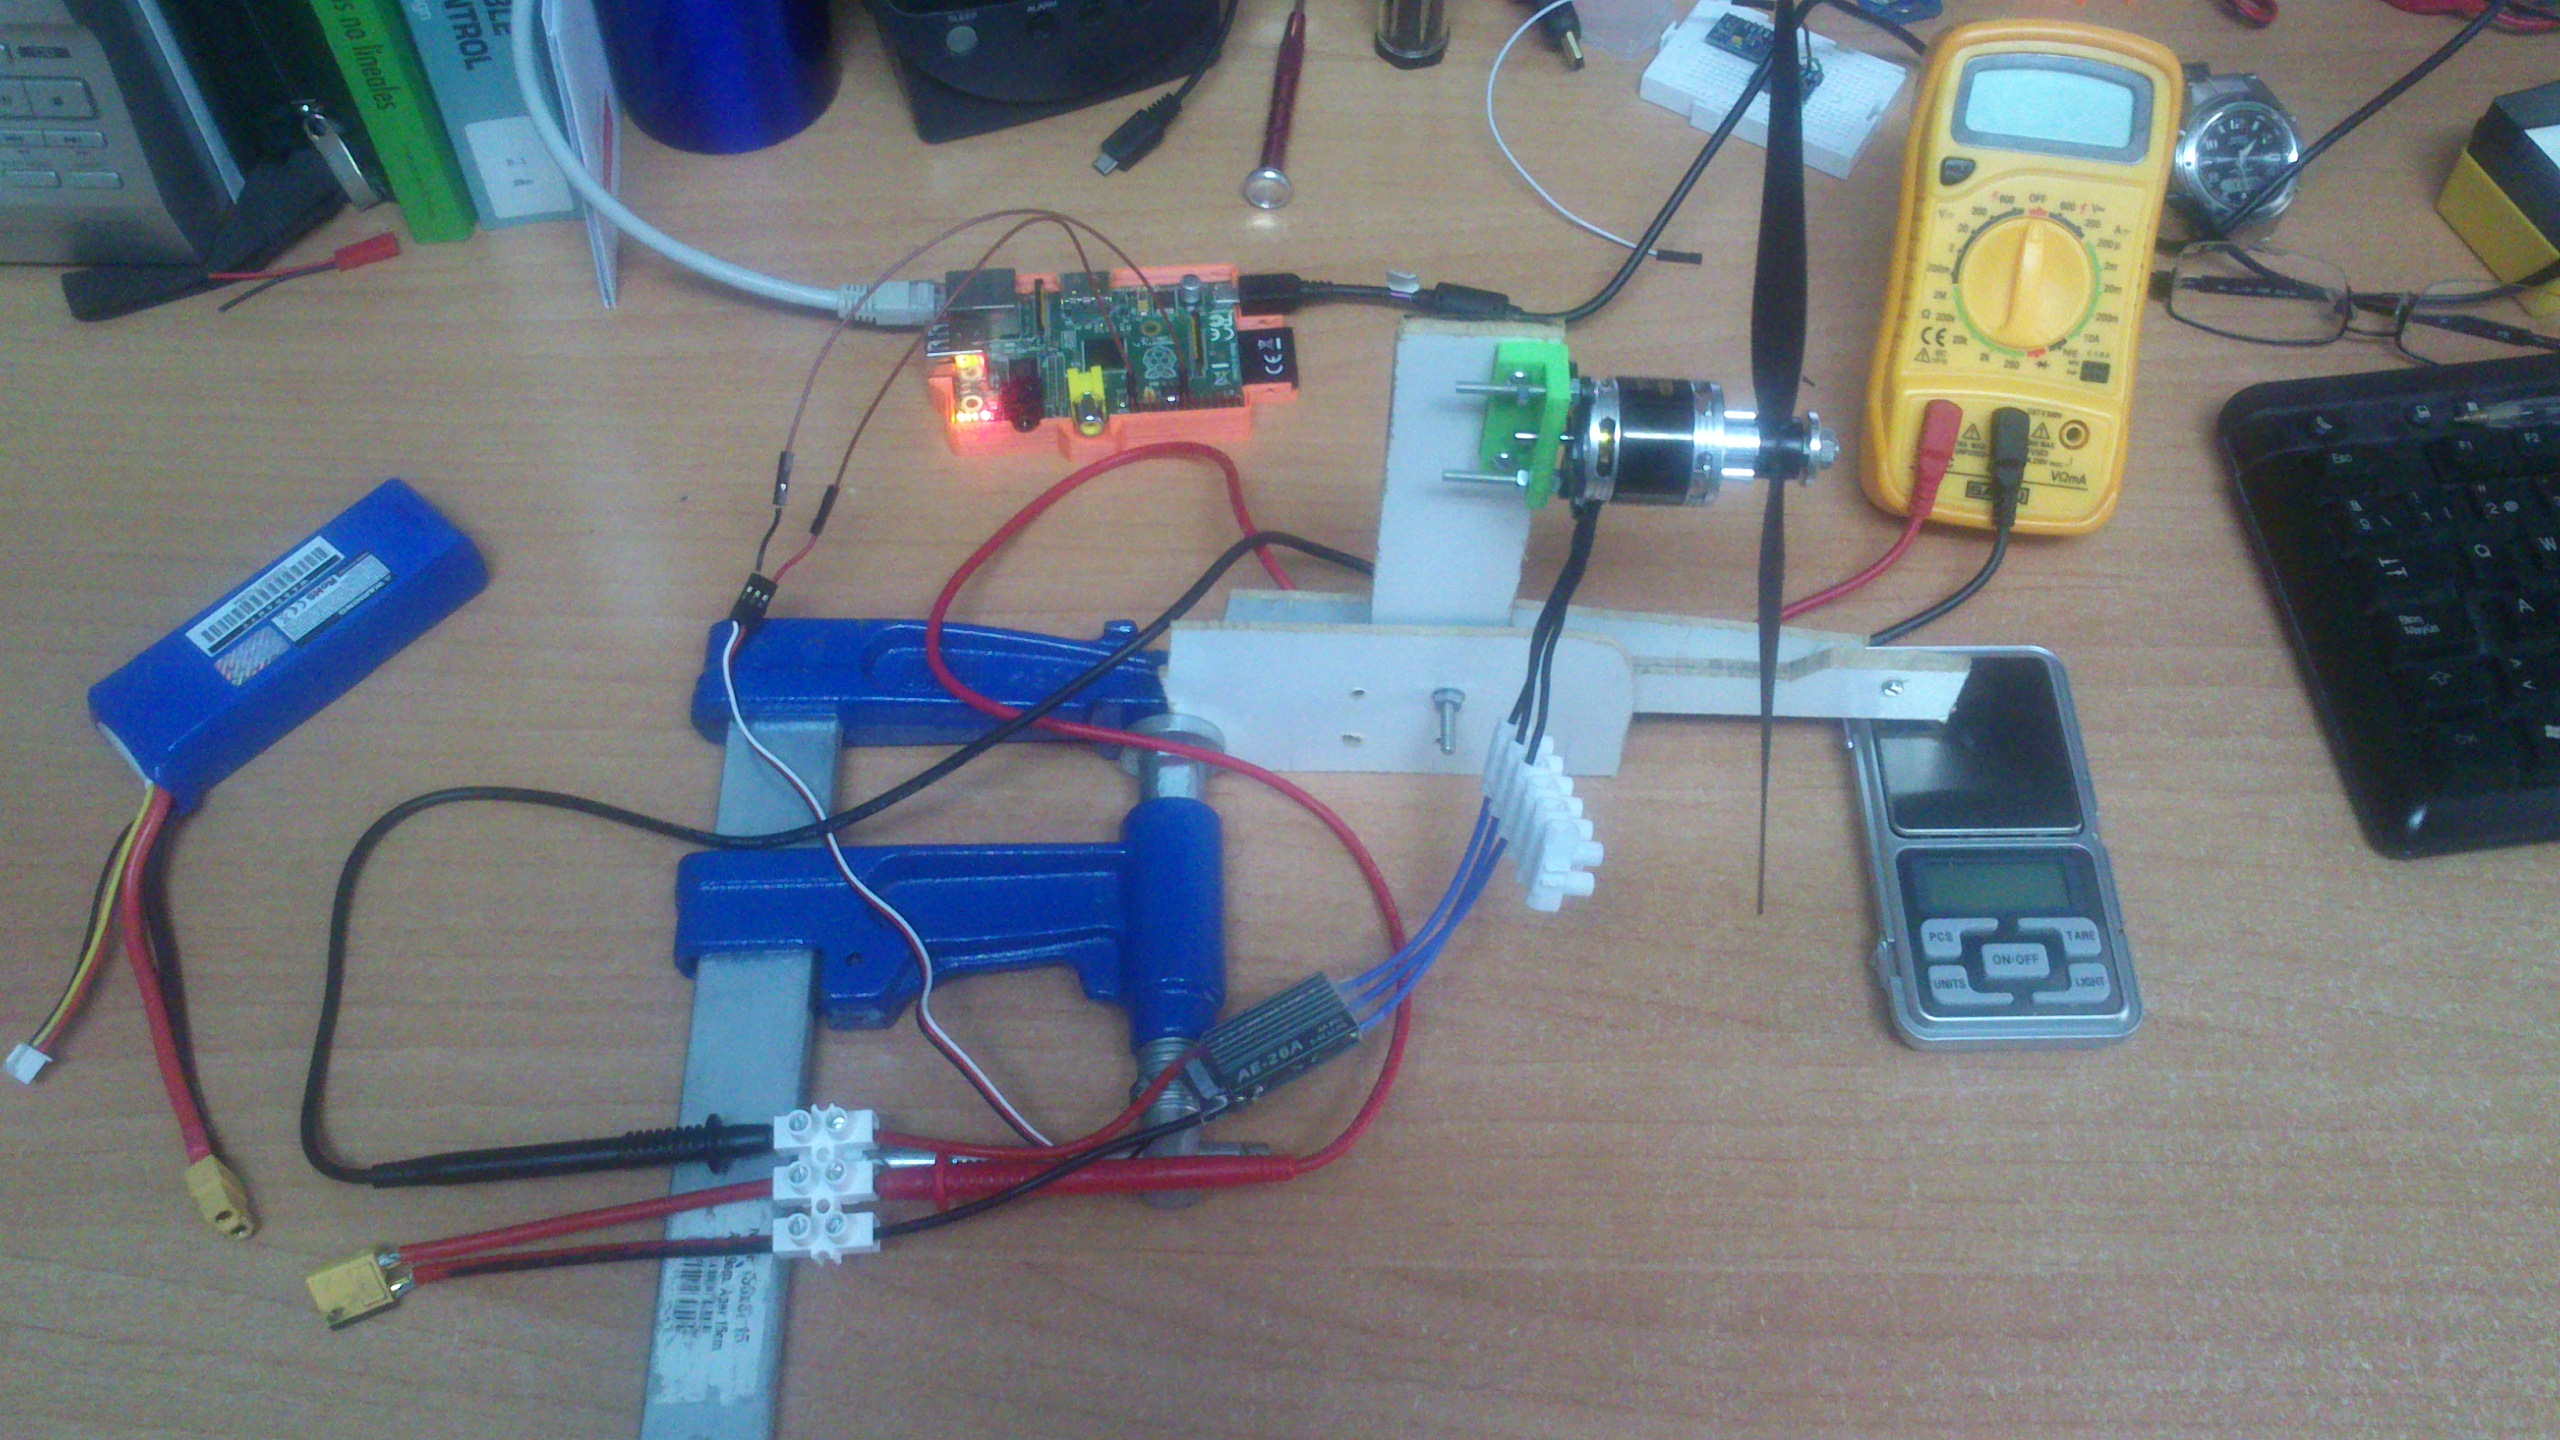
\includegraphics[scale=0.09]{images/montaje.jpg}
\caption{Montatge per a l'estudi del motor}
\end{center}
\end{figure}

Es transmet al ESC a quina velocitat s'ha de fer funcionar al motor des de la Raspberry Pi per mitjà d'una senyal PWM. El programa que s'executa per a fer les proves és:

\begin{verbatim}
#include <stdio.h>
#include <termios.h>
#include <wiringPi.h>
#include <unistd.h>

#define PIN 2 // pin 13

int main(void){

        int i,p;
        wiringPiSetup();

        pinMode(PIN,OUTPUT);
        digitalWrite(PIN,LOW);

        for(i=0;i<=100;i+=5){
                for(p=0;p<250;p++){
                        digitalWrite(PIN,HIGH);
                        delayMicroseconds(950+i*10);
                        digitalWrite(PIN,LOW);
                        delayMicroseconds(19050-i*10);

                        printf("PWM(i): %d \t h:%d \n",i,p);
                }
        }
        return 0;
}
\end{verbatim}

S'obté una mesura de força i d'intensitat per cada increment del 0.25\% del PWM enviat al Variador. Sobté:

\begin{figure}[h!]
\begin{center}
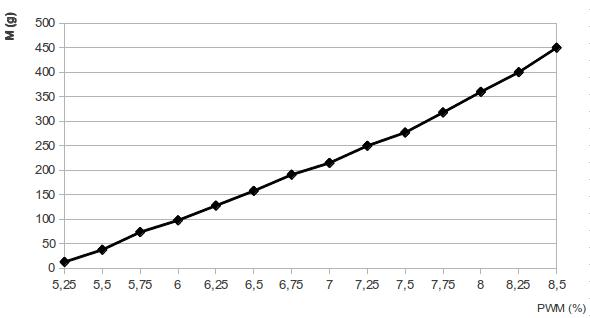
\includegraphics[scale=0.8]{images/MvsPWM.jpeg}
\caption{Relació entre la força (en grams) i el PWM}
\end{center}
\end{figure}

\begin{tikzpicture}
\begin{axis}
% \addplot plot[scale=0.8,domain=0:3.14](\x,{sin(\x r)});%r=radianes
\end{axis}
\end{tikzpicture}

En l'eix de les abscises el PWM(\%) és entre el 5\% i el 10\% de la senyal enviada, que correspon al mínim i màxim que el motor. Com que per a un PWM elevat la força era massa gran i no es preveu que es farà funcionar el sistema en semblants condicions de treball, no s'estudia. 

Es veu una relació proporcional del PWM amb la força generada. Es considera que una regressió lineal serà suficient. S'obté que la força $f(PWM)$ del motor serà:
$$f=32.5758 \cdot PWM(\%)-32.1758$$
amb un coeficient de determinació en la regressió és de  $R^2=0.9929$. Aquest resultat facilita el problema en ser una relació prou senzilla.

Per a l'intensitat es té una relació tan amigable com en el cas anterior, però com que no serà cas d'estudi, només es veurà una aproximació del que pot arribar a consumir cada motor per a assegurar una autonomía de vol no irrisòria. Es té que 
\newpage
\begin{figure}[!h]
\begin{center}
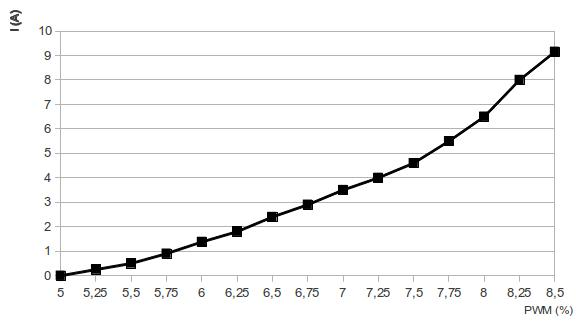
\includegraphics[scale=0.8]{images/IvsPWM.jpeg}
\caption{Relació entre la corrent consumida i el PWM}
\end{center}
\end{figure}

Com que en el punt d'equilibri cada motor suporta una cuarta part del pes, el PWM hauría de correspondre a una força de $m_{Quadcopter}\cdot g/4\approx0.225$kg. El consum corresponent és de $3.5$A aproximadament. Entre els quatre motors es consumiràn $3.5 \cdot 4=14$A. Com que la bateria es de 2200mAh es suposa una autonomia de 7 minuts aproximadament. 


\end{document}